\documentclass[lettersize,journal]{IEEEtran}
\usepackage{amsmath,amsfonts,amssymb}
\usepackage{algorithmic}
\usepackage{array}
\usepackage[caption=false,font=normalsize,labelfont=sf,textfont=sf]{subfig}
\usepackage{textcomp}
\usepackage{stfloats}
\usepackage{url}
\usepackage{verbatim}
\usepackage{graphicx}
\usepackage{cite}
\usepackage{booktabs}
\usepackage{bm}

\begin{document}

\title{Physics-Constrained Dynamic Identification and Noise Estimation for Underactuated Systems}

\author{Ahmed~Asker,
        Omar~Salah,
        and~Haitham~El-Hussieny%
\thanks{Ahmed Asker and Haitham El-Hussieny are with the Department of Mechatronics and Robotics Engineering, Egypt-Japan University of Science and Technology (E-JUST), New Borg El-Arab City, Alexandria 21934, Egypt (e-mail: ahmed.asker@ejust.edu.eg, haitham.elhussieny@ejust.edu.eg).}%
\thanks{Ahmed Asker is also with the Department of Production Engineering and Mechanical Design, Faculty of Engineering, Mansoura University, Mansoura 35516, Egypt.}%
\thanks{Omar Salah is with the Mechatronics Engineering Department, Faculty of Engineering, Assiut University, Assiut 71516, Egypt (e-mail: omar.salah@aun.edu.eg).}%
\thanks{*Corresponding author: Ahmed Asker (e-mail: ahmed.asker@ejust.edu.eg).}%
}

%\markboth{}%
%{Asker \MakeLowercase{\textit{et al.}}: Physics-Constrained Dynamic Identification and Noise Estimation for Underactuated Systems}

\maketitle

\begin{abstract} 
Dynamic identification of underactuated mechanical systems is inherently an ill-posed problem, as passive degrees of freedom (DOFs) introduce parameter degeneracy in unconstrained least-squares methods, often resulting in non-physical parameter estimates. This paper presents a physics-constrained, data-driven modeling framework based on CasADi algorithmic differentiation, where computational graphs of the Euler-Lagrange dynamics are leveraged to automatically enforce inertia symmetry, positive definiteness, and passivity constraints without requiring manual symbolic derivations. A nonlinear friction model and a Maximum Likelihood Estimation (MLE) framework are further integrated to jointly estimate both the physical parameters and sensor noise variance. Furthermore, the momentum-filtered dynamic model (dynamic filtered regression) is compared with the proposed method. The results demonstrate that, although momentum filtering eliminates the need for numerical acceleration differentiation, unconstrained filtered regression remains vulnerable to parameter degeneracy in the presence of measurement noise. In contrast, the proposed framework effectively mitigates this limitation, achieving a parameter error of 0.19\%, compared with 80.06\% for Unconstrained Momentum-Filtered Least Squares (UMF-LS) and 80.01\% for Unconstrained Direct Least Squares (U-LS) on a 3-DOF Double Inverted Pendulum on a Cart (DIPC). The proposed approach also estimates sensor noise variance with an error of only 1.36\% relative to the true value and demonstrates superior simulation accuracy on both simulated and experimental datasets of the Rotational Inverted Furuta Pendulum (RIFP). The proposed framework enables accurate and physically consistent identification of underactuated systems, supporting more reliable model-based simulation, control, and optimization in practical robotic applications.
\end{abstract} 

\begin{IEEEkeywords}
Filtered dynamic model, dynamic system identification, underactuated robotics, SINDy, Algorithmic Differentiation, nonlinear optimization.
\end{IEEEkeywords}

\section{Introduction}
\IEEEPARstart{P}{recise} dynamic models of robotic manipulators are crucial for their analysis, design optimization, and model-based control \cite{Tsai.1999, Spong2020}. High-fidelity simulation environments such as MSC ADAMS, Gazebo, and MATLAB/Simscape Multibody enable accurate numerical simulation of complex robotic systems. However, these tools do not provide compact analytical equations of motion for direct use in model-based control design. Instead, control synthesis typically relies on user-supplied dynamic models or linearized approximations generated around operating points. As a result, controller performance may deteriorate when the system operates far from the linearization region or experiences strong nonlinearities. The ability of these simulation environments to generate large volumes of state and input-output data has motivated growing interest in data-driven methods for identifying analytical dynamic models directly from data \cite{omar2022framework,omar2024robust,omar2025r,Karniadakis2021}.

Robot dynamic models are traditionally obtained through either first-principles modeling or data-driven approaches. First-principles methods derive the equations of motion from analytical mechanics, typically using Euler-Lagrange or Newton-Euler formulations. These models preserve the physical structure of the system and provide valuable insight into its dynamics; however, their development for complex multi-link mechanisms can be labor-intensive and susceptible to modeling errors. Moreover, practical implementation often requires accurate identification of inertial, geometric, and friction parameters, introducing an additional layer of complexity. Consequently, advances in machine learning, optimization, and computational mechanics have stimulated growing interest in data-driven approaches that simultaneously address dynamic model discovery and parameter identification directly from experimental data \cite{hashemi2023multibody, StevenL.Brunton.2016, NguyenTuong2011}.

The potential of data-driven learning to generate interpretable white-box analytical models has attracted considerable interest in recent years. Unlike black-box approaches, such as neural networks, which often provide limited physical insight, interpretable methods including Sparse Identification of Nonlinear Dynamics (SINDy) and its parallel implicit variant, SINDy-PI, seek to identify parsimonious governing equations directly from data by selecting a small subset of active basis functions from large candidate libraries \cite{StevenL.Brunton.2016, Kaheman.2020,omar2024robust}. These sparse-regression and library-based identification techniques have demonstrated promising performance in robotic applications. For instance, Chen et al. \cite{Chen.2021} employed SINDy with Lasso regression to identify the dynamics of a three-degree-of-freedom (3-DOF) manipulator for trajectory planning. Similarly, \cite{omar2022framework} proposed a data-driven framework for discovering the dynamics of planar serial manipulators. Subsequently, \cite{omar2024robust} introduced a robust dynamic model discovery methodology for fully actuated industrial manipulators using simple, non-optimal excitation trajectories. In that work, unknown geometric and inertial parameters were represented symbolically and embedded within an Euler-Lagrange-based candidate library. By enforcing physical constraints across multiple excitation trajectories, the proposed framework substantially reduced sensitivity to regressor matrix conditioning and mitigated the traditional dependence on mathematically optimal excitation trajectories.

Despite these advances, interpretable data-driven modeling methods have been developed almost exclusively for fully actuated manipulators \cite{Kaheman.2020, Chu.2020, omar2024robust}. In contrast, underactuated robotic systems, characterized by having fewer independent actuators than generalized degrees of freedom (DOFs), are still predominantly modeled using black-box neural networks or non-parametric Gaussian process frameworks \cite{sintov2019learning, wang2022data}. The dynamics of underactuated systems are inherently nonlinear due to the strong coupling between actuated and passive coordinates. Rather than directly actuating all DOFs, these systems exploit passive dynamics to improve energy efficiency, agility, and mechanical compliance, making them attractive for applications such as legged locomotion, aerial manipulation, and assistive robotics \cite{yang2023concurrent, Fantoni2002}. However, the same characteristics that make underactuated systems attractive also introduce significant challenges for system identification.

Since passive joints are unactuated, the associated identification problem becomes homogeneous, often leading to severely ill-conditioned regression matrices. As a result, unconstrained least-squares methods may drive passive parameters toward zero in the presence of measurement noise or differentiation errors, producing physically meaningless estimates with vanishing masses and inertias \cite{Asker2024}. Underactuated systems also exhibit non-integrable dynamic constraints that couple passive and actuated coordinates through inertial, Coriolis, and gravitational effects, preventing independent control of passive motions \cite{Fantoni2002}. In addition, excitation design is inherently restricted, as passive coordinates cannot be independently excited and excessive excitation can destabilize the system, limiting the informativeness of experimental data \cite{Swevers2007, AguilarSierra2014}. Finally, unconstrained identification may yield non-physical inertia matrices that violate positive definiteness, leading to numerical instability and simulation divergence during forward integration \cite{Traversaro2016, Mehta2023}.

While hybrid rigid-body neural network dynamics \cite{Lutter2019, Hwangbo2019, Lee2024} and Physics-Informed Neural Networks (PINNs) \cite{Raissi2019, Karniadakis2021} have been proposed to merge physics with learning, they introduce millisecond-scale neural evaluation latencies that impede high-frequency (1--2~kHz) embedded real-time execution in closed-loop nonlinear model predictive control (NMPC). Furthermore, penalty-based physics-informed losses treat physical conservation laws as soft penalties, offering no mathematical guarantee that the estimated inertia matrix remains strictly positive definite across the entire configuration space \cite{Mehta2023, Schillinger2024}.

Crucially, existing acceleration-free regression formulations, such as the classical Unconstrained Momentum-Filtered Least Squares (UMF-LS) baseline \cite{GarciaAlarcon2012, AguilarSierra2014}, filter dynamic equations with linear low-pass operators to construct a filtered dynamic model that bypasses numerical acceleration differentiation. However, linear filtering remains an unconstrained transformation that lacks cross-subsystem physical coupling constraints. Under noisy measurements, unconstrained momentum filtering fails to prevent parameter degeneration in passive coordinates and overfits training data without statistically estimating true sensor noise variance. To bridge these gaps, a preliminary Physics-Constrained Least Squares (PC-LS) concept was introduced in \cite{Asker2024}, showing that physical constraints can eliminate parameter degeneration.

In this paper, the physics-constrained methodology in \cite{omar2024robust} and preliminary formulations \cite{Asker2024} are substantially advanced and generalized to resolve the unique pathologies of underactuated mechanical systems. We formally generalize the momentum-filtered dynamic model (dynamic filtered regression) to underactuated systems. Rather than solving the equations of motion for each link separately, we formulate the underactuated identification problem in a unified, stacked matrix architecture solved in a single global step. The physical constraints are derived systematically from the fundamental conservation properties of multi-body dynamics.

The primary contributions of this paper are summarized as follows: 
\begin{itemize} 
	\item \textbf{Physics-Constrained Identification Framework:} An end-to-end identification framework based on computational directed acyclic graphs (DAGs) in algorithmic differentiation and implemented using CasADi \cite{Andersson2019}. The framework automatically generates inverse-dynamics regressors and extracts fundamental physical constraints, eliminating the need for manual symbolic derivations.
	 
	\item \textbf{Simultaneous Parameter and Noise-Variance Estimation:} A Maximum Likelihood Estimation (MLE) framework is formulated to jointly identify dynamic and friction parameters alongside sensor noise variance. Beyond providing a measure of identification quality, the estimated noise variance directly parameterizes measurement covariances in dynamic observers and state estimators. By exploiting normal-equation sufficient statistics, the optimization problem is reduced to a compact form that can be solved efficiently \cite{Wachter2006}.

	\item \textbf{Open-Source Algorithmic Implementation and Benchmarking Suite:} To promote reproducible research and facilitate community benchmarking in underactuated robotics, all algorithmic differentiation computational graphs, multi-body simulation testbeds, experimental datasets, and replication scripts are made publicly available in the open-source companion repository \cite{AskerRepo2026}.
\end{itemize}

%The remainder of this paper is structured as follows. Section~\ref{sec:dynamics} establishes the underactuated Euler-Lagrange equations of motion, fundamental physical conservation laws, the general derivation of the acceleration-free dynamic filtered regressor, and the concrete dynamic and filtered formulations for both the 3-DOF DIPC (controlled stochastic simulation benchmark with known ground truth) and 2-DOF RIFP (physical hardware benchmark subjected to quantization noise, bearing friction, and truncated observation horizons). Section~\ref{sec:casadi_engine} details the algorithmic differentiation engine, automated constraint extraction, nonlinear friction formulation, and the condensed MLE framework. Section~\ref{sec:benchmarks_setup} outlines the simulation and experimental benchmarking protocols, sensor noise injection, the RIFP experimental dataset from \cite{AguilarSierra2014}, and comparative methodologies. Section~\ref{sec:results} presents the comprehensive results and in-depth physical, statistical, and computational discussions across both testbeds. Finally, Section~\ref{sec:conclusion} concludes the paper.

\section{Dynamic Modeling of Underactuated Mechanical Systems}
\label{sec:dynamics}
This section establishes the theoretical foundations of physics-constrained parameter identification and presents the dynamic modeling framework for underactuated robotic systems \cite{Fantoni2002, Asker2024}. The partitioned Euler-Lagrange equations of motion and the fundamental physical properties of mechanical systems, namely generalized inertia symmetry, strict positive definiteness, and passivity-induced skew-symmetry, are first formulated \cite{Slotine1987, Spong2020, Bargsten2023}. To avoid the severe noise amplification associated with numerical acceleration differentiation, an acceleration-free filtered dynamic regressor is then derived through generalized momentum decomposition and causal low-pass filtering \cite{Reyes1997, GarciaAlarcon2012, AguilarSierra2014}. Although the analytical derivation of filtered dynamic regressors becomes increasingly intractable for high-degree-of-freedom systems due to the combinatorial growth of Christoffel tensor terms \cite{Gautier1990}, representing multibody dynamics as computational graphs enables their automatic extraction through algorithmic differentiation and analytical derivative algorithms \cite{Andersson2019, Carpentier2018, Carpentier2019}. The framework is subsequently instantiated on two underactuated benchmark systems with distinct kinematic topologies: the 3-DOF translationally driven Double Inverted Pendulum on a Cart (DIPC) \cite{Asker2024} and the 2-DOF rotationally driven Rotational Inverted Furuta Pendulum (RIFP) \cite{AguilarSierra2014}. For each platform, both the standard linear-in-the-parameters (LIP) representation and the corresponding filtered dynamic regressor are derived.

\subsection{Euler-Lagrange Dynamics and Fundamental Physical Properties}
Consider an $n$-DOF robotic mechanism described by generalized coordinates $\bm{q} \in \mathbb{R}^n$ and velocities $\dot{\bm{q}} \in \mathbb{R}^n$. The equations of motion governed by Lagrangian mechanics are expressed as:
\begin{equation}
    D(\bm{q})\ddot{\bm{q}} + C(\bm{q}, \dot{\bm{q}})\dot{\bm{q}} + \bm{G}(\bm{q}) + \bm{\tau}_f(\dot{\bm{q}}) = \bm{\tau},
    \label{eq:eom}
\end{equation}
where $D(\bm{q}) \in \mathbb{R}^{n \times n}$ represents the symmetric, positive-definite generalized inertia matrix; $C(\bm{q}, \dot{\bm{q}}) \in \mathbb{R}^{n \times n}$ is the Coriolis and centrifugal matrix; $\bm{G}(\bm{q}) \in \mathbb{R}^n$ is the gravitational torque vector; $\bm{\tau}_f(\dot{\bm{q}}) \in \mathbb{R}^n$ models joint friction forces and torques; and $\bm{\tau} \in \mathbb{R}^n$ is the generalized actuation torque vector.

For an underactuated system possessing $m$ actuated coordinates and $p = n - m$ passive joints, the generalized coordinates and actuation vectors are partitioned as:
\begin{equation}
    \bm{q} = \begin{bmatrix} \bm{q}_a \\ \bm{q}_u \end{bmatrix}, \quad \bm{\tau} = \begin{bmatrix} \bm{\tau}_a \\ \mathbf{0}_{p \times 1} \end{bmatrix},
    \label{eq:partition}
\end{equation}
where $\bm{q}_a \in \mathbb{R}^m$ and $\bm{q}_u \in \mathbb{R}^p$ denote the actuated and passive DOFs, respectively, and the generalized torques associated with the passive joints are identically zero ($\bm{\tau}_u = \mathbf{0}$).

Partitioning the equations of motion in \eqref{eq:eom} according to the coordinate decomposition in \eqref{eq:partition} yields
\begin{equation}
	\begin{bmatrix}
		D_{aa}(\bm{q}) & D_{au}(\bm{q}) \\
		D_{ua}(\bm{q}) & D_{uu}(\bm{q})
	\end{bmatrix}
	\begin{bmatrix}
		\ddot{\bm{q}}_a \\
		\ddot{\bm{q}}_u
	\end{bmatrix}
	+
	\begin{bmatrix}
		\bm{h}_a(\bm{q},\dot{\bm{q}}) \\
		\bm{h}_u(\bm{q},\dot{\bm{q}})
	\end{bmatrix}
	=
	\begin{bmatrix}
		\bm{\tau}_a \\
		\mathbf{0}_{p\times1}
	\end{bmatrix},
	\label{eq:partitioned_eom}
\end{equation}
where $\bm{\tau}_a \in \mathbb{R}^{m}$ denotes the vector of actuator torques applied to the actuated coordinates, while the passive coordinates receive no direct actuation.

The dynamics associated with the unactuated coordinates satisfy the following acceleration-level constraint: 
\begin{equation}
    D_{ua}(\bm{q})\ddot{\bm{q}}_a + D_{uu}(\bm{q})\ddot{\bm{q}}_u + \bm{h}_u(\bm{q}, \dot{\bm{q}}) = \mathbf{0}_{p \times 1}.
    \label{eq:nonholonomic_constraint}
\end{equation}
Because \eqref{eq:nonholonomic_constraint} cannot be integrated into geometric coordinates, the passive motions are nonlinearly coupled to the actuated coordinates \cite{Fantoni2002}. Expressing the dynamic model in LIP form yields the partitioned regression system:
\begin{equation}
    \begin{bmatrix} W_a(\bm{q}, \dot{\bm{q}}, \ddot{\bm{q}}) \\ W_u(\bm{q}, \dot{\bm{q}}, \ddot{\bm{q}}) \end{bmatrix} \bm{\Theta} = \begin{bmatrix} \bm{\tau}_a \\ \mathbf{0}_{p \times 1} \end{bmatrix}.
    \label{eq:partitioned_regressor}
\end{equation}

Because the external generalized force acting on the unactuated joints is identically zero, the regression sub-problem corresponding to the passive coordinates is strictly homogeneous:
\begin{equation}
    W_u(\bm{q}, \dot{\bm{q}}, \ddot{\bm{q}}) \bm{\Theta}_u \approx \mathbf{0},
    \label{eq:nullspace_subsystem}
\end{equation}
where $\bm{\Theta}_u$ collects the parameter subset governing the passive links. When solved via unconstrained direct least squares (U-LS), the normal matrix $W_u^T W_u$ is often severely ill-conditioned. In the presence of sensor noise, encoder quantization, or numerical acceleration differentiation errors, unconstrained solvers trivially minimize algebraic residuals by driving the passive parameters toward the trivial solution ($\bm{\Theta}_u \to \mathbf{0}$). This results in the complete loss of estimated mass and inertia for passive links, rendering the identified model physically meaningless.

Mechanical systems governed by \eqref{eq:eom} inherently satisfy three fundamental properties:

\noindent\textbf{Property 1 (Inertia Symmetry):} The generalized inertia matrix is symmetric across the configuration space:
\begin{equation}
	D(\bm{q}) = D^T(\bm{q}), \quad \forall \bm{q} \in \mathbb{R}^n.
	\label{eq:prop_sym}
\end{equation}

\noindent\textbf{Property 2 (Inertia Positive Definiteness):} The generalized inertia matrix is strictly positive definite and uniformly bounded:
\begin{equation}
	0 < \lambda_{\min} I \preceq D(\bm{q}) \preceq \lambda_{\max} I, \quad \forall \bm{q} \in \mathbb{R}^n.
	\label{eq:prop_pd}
\end{equation}
Equivalently, strict positive definiteness holds if and only if all leading principal minors of the inertia matrix are strictly positive, $\Delta_k(D(\bm{q})) > 0$, $k = 1, \dots, n$.

\noindent\textbf{Property 3 (Passivity Skew-Symmetry):} When the Coriolis and centrifugal matrix $C(\bm{q}, \dot{\bm{q}})$ is defined as follows:
\begin{equation}
	C_{ij}(\bm{q}, \dot{\bm{q}}) = \sum_{k=1}^n \frac{1}{2} \left( \frac{\partial D_{ij}}{\partial q_k} + \frac{\partial D_{ik}}{\partial q_j} - \frac{\partial D_{jk}}{\partial q_i} \right) \dot{q}_k,
	\label{eq:christoffel}
\end{equation}
the matrix $N(\bm{q}, \dot{\bm{q}})=\dot{D}(\bm{q}, \dot{\bm{q}})-2C(\bm{q}, \dot{\bm{q}})$ is skew-symmetric, satisfying 
\begin{equation*}
	N(\bm{q}, \dot{\bm{q}})+N^{T}(\bm{q}, \dot{\bm{q}})=\mathbf{0}_{n\times n}
\end{equation*}
which holds if and only if its elements $n_{ij}(\bm{q}, \dot{\bm{q}})$ satisfy the entrywise algebraic conditions:
\begin{equation}
	n_{ij} + n_{ji} = 0, \quad \forall i, j \in \{1, \dots, n\}.
	\label{eq:skew_entrywise}
\end{equation}
Evaluating \eqref{eq:skew_entrywise} yields two distinct sets of equality constraints:
\begin{align}
	n_{ij} &= 0, & \text{for } i = j, \label{eq:skew_diag} \\
	n_{ij} &= -n_{ji}, & \text{for } i \neq j. \label{eq:skew_offdiag}
\end{align}

\subsection{Derivation of the Acceleration-Free Dynamic Filtered Regressor} \label{sec:filtered_derivation}
A prominent challenge in dynamic parameter identification is that conventional inverse-dynamics regression models depend explicitly on generalized joint accelerations $\ddot{\bm{q}}$. In physical robotic systems, accelerations are rarely measured directly and must be approximated via numerical differentiation of noisy encoder positions, introducing severe high-frequency noise that degrades parameter estimation accuracy.

To address this challenge without relying on numerical differentiation of acceleration signals, this section establishes the acceleration-free filtered dynamic model (dynamic filtered regression) \cite{GarciaAlarcon2012, AguilarSierra2014, Reyes1997}. Consider the generalized momentum vector of an $n$-DOF mechanical system, defined as
\begin{equation}
	\bm{p}(\bm{q}, \dot{\bm{q}}) = D(\bm{q})\dot{\bm{q}}.
	\label{eq:momentum_def}
\end{equation}
Differentiating \eqref{eq:momentum_def} with respect to time yields:
\begin{equation}
	\frac{d}{dt} \bm{p}(\bm{q}, \dot{\bm{q}}) = D(\bm{q})\ddot{\bm{q}} + \dot{D}(\bm{q}, \dot{\bm{q}})\dot{\bm{q}}.
	\label{eq:momentum_diff}
\end{equation}
Rearranging \eqref{eq:momentum_diff} for the inertial acceleration term $D(\bm{q})\ddot{\bm{q}}$ and substituting into the Euler-Lagrange equations \eqref{eq:eom} gives:
\begin{equation}
	\frac{d}{dt}\left(D(\bm{q})\dot{\bm{q}}\right) + \left[C(\bm{q}, \dot{\bm{q}}) - \dot{D}(\bm{q}, \dot{\bm{q}})\right]\dot{\bm{q}} + \bm{G}(\bm{q}) + \bm{\tau}_f(\dot{\bm{q}}) = \bm{\tau}.
	\label{eq:momentum_eom}
\end{equation}
Because both the momentum vector $D(\bm{q})\dot{\bm{q}}$ and the residual dynamic terms are linear in the identifiable parameter vector $\bm{\Theta}$, \eqref{eq:momentum_eom} factorizes into two separate linear regressor matrices:
\begin{align}
	D(\bm{q})\dot{\bm{q}} &= \Omega_a(\bm{q}, \dot{\bm{q}}) \bm{\Theta}, \label{eq:omega_a} \\
	\left[C(\bm{q}, \dot{\bm{q}}) - \dot{D}(\bm{q}, \dot{\bm{q}})\right]\dot{\bm{q}} + \bm{G}(\bm{q}) + \bm{\tau}_f(\dot{\bm{q}}) &= \Omega_b(\bm{q}, \dot{\bm{q}}) \bm{\Theta}. \label{eq:omega_b}
\end{align}
Substituting \eqref{eq:omega_a} and \eqref{eq:omega_b} into \eqref{eq:momentum_eom} establishes the canonical momentum-residual decomposition \cite{GarciaAlarcon2012, AguilarSierra2014}:
\begin{equation}
	\frac{d}{dt}\left[\Omega_a(\bm{q}, \dot{\bm{q}})\bm{\Theta}\right] + \Omega_b(\bm{q}, \dot{\bm{q}})\bm{\Theta} = \bm{\tau}.
	\label{eq:filtered_decomp}
\end{equation}

To eliminate the explicit time-derivative operator $\frac{d}{dt}$ without computing numerical derivatives, a stable first-order low-pass filter $f(s) = \frac{\lambda}{s + \lambda}$ with cutoff bandwidth $\lambda > 0$ is applied to both sides of \eqref{eq:filtered_decomp} in the Laplace domain:
\begin{equation}
	\left[ s f(s)\Omega_a(\bm{q}, \dot{\bm{q}}) + f(s)\Omega_b(\bm{q}, \dot{\bm{q}}) \right]\bm{\Theta} = f(s)\bm{\tau}.
	\label{eq:filtered_laplace}
\end{equation}
Transforming back to the time domain, the filtered regressor components are defined as:
\begin{align}
	\Omega_{af}(\bm{q}, \dot{\bm{q}}) &= \mathcal{L}^{-1}\left\{ s f(s)\Omega_a(\bm{q}, \dot{\bm{q}}) \right\}, \label{eq:omega_af} \\
	\Omega_{bf}(\bm{q}, \dot{\bm{q}}) &= \mathcal{L}^{-1}\left\{ f(s)\Omega_b(\bm{q}, \dot{\bm{q}}) \right\}, \label{eq:omega_bf} \\
	\bm{\tau}_{\text{filt}} &= \mathcal{L}^{-1}\left\{ f(s)\bm{\tau} \right\}. \label{eq:tau_filt_def}
\end{align}
The operator $s f(s) = \frac{\lambda s}{s + \lambda}$ acts as a proper, strictly causal bandpass filter that differentiatively convolutes $\Omega_a(\bm{q}, \dot{\bm{q}})$ while attenuating high-frequency noise above bandwidth $\lambda$. By defining the total dynamic filtered regressor as:
\begin{equation}
	\Omega_f(\bm{q}, \dot{\bm{q}}) = \Omega_{af}(\bm{q}, \dot{\bm{q}}) + \Omega_{bf}(\bm{q}, \dot{\bm{q}}),
	\label{eq:total_omega_f}
\end{equation}
the linear, acceleration-free filtered regression model is obtained:
\begin{equation}
	\Omega_f(\bm{q}, \dot{\bm{q}})\bm{\Theta} = \bm{\tau}_{\text{filt}}.
	\label{eq:dynamic_filtered_model}
\end{equation}

For discrete-time implementation at sampling period $T_s$, the continuous transfer functions $s f(s)$ and $f(s)$ are discretized into digital Infinite Impulse Response (IIR) filters:
\begin{align}
	H_D(z) &= \frac{\lambda(1 - z^{-1})}{1 - e^{-\lambda T_s} z^{-1}}, \label{eq:discrete_diff} \\
	H_L(z) &= \frac{1 - e^{-\lambda T_s}}{1 - e^{-\lambda T_s} z^{-1}}. \label{eq:discrete_lowpass}
\end{align}

Under the coordinate partitioning \eqref{eq:partition} for underactuated mechanisms, the filtered torque vector decomposes as $\bm{\tau}_{\text{filt}} = [\bm{\tau}_{a,\text{filt}}^T, \mathbf{0}_{p \times 1}^T]^T$. Consequently, the filtered regression system partitions into actuated and passive blocks:
\begin{equation}
	\begin{bmatrix} \Omega_{f,a}(\bm{q}, \dot{\bm{q}}) \\ \Omega_{f,u}(\bm{q}, \dot{\bm{q}}) \end{bmatrix} \bm{\Theta} = \begin{bmatrix} \bm{\tau}_{a,\text{filt}} \\ \mathbf{0}_{p \times 1} \end{bmatrix},
	\label{eq:partitioned_filtered_regressor}
\end{equation}
where the passive subsystem equations $\Omega_{f,u}(\bm{q}, \dot{\bm{q}})\bm{\Theta} \approx \mathbf{0}$ remain strictly homogeneous.
\subsection{Underactuated Double Inverted Pendulum on a Cart (DIPC)}
\label{sec:dipc_modeling}
The first benchmark system investigated is the 3-DOF underactuated DIPC. The mechanism comprises an actuated prismatic cart of mass $m_1$ moving horizontally with displacement $d_1$, upon which two passive revolute pendulum links of masses $m_2, m_3$, lengths $a_2, a_3$, and moments of inertia $I_{2zz}, I_{3zz}$ are serially attached. The generalized coordinate vector is $\bm{q} = [d_1, \theta_2, \theta_3]^T \in \mathbb{R}^3$, and the generalized force vector is $\bm{\tau} = [F_1, 0, 0]^T \in \mathbb{R}^3$, where $F_1$ is the external force applied to the cart and the passive joint torques are identically zero ($\tau_2 = 0, \tau_3 = 0$).

\begin{figure}[t]
    \centering
    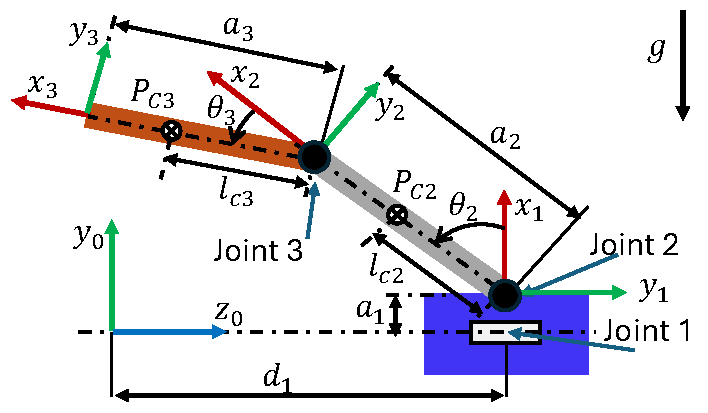
\includegraphics[width=0.88\linewidth]{figures/Sys_DH.pdf}
    \caption{Schematic and coordinate frame assignments for the 3-DOF underactuated DIPC according to the Denavit-Hartenberg (DH) convention.}
    \label{fig:dipc_schematic}
\end{figure}

\begin{table}[t]
\centering
\caption{Kinematic and Inertial Parameters for the 3-DOF Underactuated DIPC System}
\label{tab:dipc_dh}
\renewcommand{\arraystretch}{1.2}
\resizebox{\columnwidth}{!}{%
\begin{tabular}{lcccccccc}
\toprule
\textbf{Link} $i$ & \textbf{Joint Type} & $\theta_i$ & $d_i$ & $\alpha_i$ & $a_i~(\mathrm{m})$ & $\bm{P}_{Ci}^T~(\mathrm{m})$ & $m_i~(\mathrm{kg})$ & $I_{izz}~(\mathrm{kg\cdot m^2})$ \\
\midrule
1 (Cart)     & Prismatic & $\pi/2$    & $d_1$ & $-\pi/2$ & $0$    & $[0, 0, 0]$     & $5.40$ & --- \\
2 (Pend. 1)  & Revolute  & $\theta_2$ & $0$   & $0$      & $0.50$ & $[0.25, 0, 0]$ & $1.35$ & $0.0284$ \\
3 (Pend. 2)  & Revolute  & $\theta_3$ & $0$   & $0$      & $0.50$ & $[0.25, 0, 0]$ & $1.35$ & $0.0284$ \\
\bottomrule
\end{tabular}%
}
\end{table}

The schematic of the system along with the coordinate frame assignments is shown in Fig.~\ref{fig:dipc_schematic}. The kinematic parameters, link center-of-mass (CoM) position vectors, and inertial properties defined under the Denavit-Hartenberg (DH) convention are summarized in Table~\ref{tab:dipc_dh}. The parameters $\theta_i, d_i, \alpha_i$, and $a_i$ define joint angles, link offsets, twists, and lengths, while $\bm{P}_{Ci} = [x_{ci}, y_{ci}, z_{ci}]^T$ defines the position of the CoM of link $i$ relative to frame $i-1$ expressed in frame $i$ \cite{Tsai.1999}. For the planar pendulums, the CoM positions lie along the link longitudinal axes at $\bm{P}_{Ci} = [lc_i, 0, 0]^T$ ($lc_2 = lc_3 = 0.25\text{ m}$), matching Fig.~\ref{fig:dipc_schematic} and Table~\ref{tab:dipc_benchmark}. The translational velocity Jacobians $\bm{J}_{v,ij}$ and rotational velocity Jacobians $\bm{J}_{\omega,ij}$ for each link $i \in \{1, 2, 3\}$ with respect to joint $j \le i$ are given by $\bm{J}_{v,11} = \bm{z}_0$ (prismatic joint), $\bm{J}_{v,ij} = \bm{z}_{j-1} \times (\bm{p}_{ci}^0 - \bm{p}_{0,j-1}^0)$ for revolute joints ($j \ge 2$), $\bm{J}_{\omega,11} = \mathbf{0}$, and $\bm{J}_{\omega,ij} = \bm{z}_{j-1}$ ($j \ge 2$), where $\bm{z}_{j-1}$ denotes the unit actuation axis of joint $j$.

Gravitational acceleration is $g = 9.80665~\text{m/s}^2$ directed along the negative vertical axis. Joint friction is modeled as frictionless ($\bm{\tau}_f(\dot{\bm{q}}) = \mathbf{0}$) in this standard benchmark to evaluate purely inertial and gravitational underactuated coupling under measurement noise.

Synthesizing kinetic and potential energy components yields the parameterized dynamic equations:
\begin{equation}
    D(\bm{q})\ddot{\bm{q}} + C(\bm{q}, \dot{\bm{q}})\dot{\bm{q}} + \bm{G}(\bm{q}) = \bm{\tau},
    \label{eq:dipc_dynamics}
\end{equation}
where the symmetric generalized inertia matrix $D(\bm{q}) \in \mathbb{R}^{3 \times 3}$ has entries:
\begin{align}
    D_{11} &= m_1 + m_2 + m_3, \label{eq:D11_dipc} \\
    D_{12} = D_{21} &= -(m_3 a_2 + m_2 lc_2)\cos(\theta_2) \nonumber \\
                    &\quad - m_3 lc_3 \cos(\theta_2 + \theta_3), \label{eq:D12_dipc} \\
    D_{13} = D_{31} &= -m_3 lc_3 \cos(\theta_2 + \theta_3), \label{eq:D13_dipc} \\
    D_{22} &= I_{2zz} + I_{3zz} + m_2 lc_2^2 + m_3 a_2^2 + m_3 lc_3^2 \nonumber \\
           &\quad + 2 m_3 a_2 lc_3 \cos(\theta_3), \label{eq:D22_dipc} \\
    D_{23} = D_{32} &= I_{3zz} + m_3 lc_3^2 + m_3 a_2 lc_3 \cos(\theta_3), \label{eq:D23_dipc} \\
    D_{33} &= I_{3zz} + m_3 lc_3^2. \label{eq:D33_dipc}
\end{align}
The Coriolis and centrifugal matrix $C(\bm{q}, \dot{\bm{q}}) \in \mathbb{R}^{3 \times 3}$ derived via \eqref{eq:christoffel} satisfies passivity skew-symmetry, and the gravitational vector is $\bm{G}(\bm{q}) = [0, -(m_2 lc_2 + m_3 a_2)g \sin(\theta_2) - m_3 lc_3 g \sin(\theta_2 + \theta_3), -m_3 lc_3 g \sin(\theta_2 + \theta_3)]^T$.

Applying the Euler-Lagrange equations yields a linear-in-the-parameters (LIP) representation for each link subsystem $i \in \{1, 2, 3\}$:
\begin{equation}
    L_i(\bm{q}, \dot{\bm{q}}, \ddot{\bm{q}}) \bm{\Theta}_{L_i} = \tau_i,
    \label{eq:dipc_link_reg}
\end{equation}
where $L_1 \in \mathbb{R}^{N \times 8}$, $L_2 \in \mathbb{R}^{N \times 10}$, and $L_3 \in \mathbb{R}^{N \times 6}$ are the analytical regressor matrices corresponding to the subsystem parameter vectors $\bm{\Theta}_{L_1} \in \mathbb{R}^8$, $\bm{\Theta}_{L_2} \in \mathbb{R}^{10}$, and $\bm{\Theta}_{L_3} \in \mathbb{R}^{6}$ compiled in Table~\ref{tab:dipc_benchmark}. The total dynamic parameter vector is $\bm{\Theta} = [\bm{\Theta}_{L_1}^T, \bm{\Theta}_{L_2}^T, \bm{\Theta}_{L_3}^T]^T \in \mathbb{R}^{24}$ (with $\bm{\Theta} = \bm{\Theta}_{\text{dyn}}$ as $\bm{\Theta}_{\text{fric}} = \mathbf{0}$). The full stacked regressor is given by:
\begin{equation}
    W = \begin{bmatrix} L_1 & \mathbf{0} & \mathbf{0} \\ \mathbf{0} & L_2 & \mathbf{0} \\ \mathbf{0} & \mathbf{0} & L_3 \end{bmatrix} \in \mathbb{R}^{3N \times 24}, \quad \bm{\Gamma} = \begin{bmatrix} \bm{F}_1 \\ \mathbf{0}_{N \times 1} \\ \mathbf{0}_{N \times 1} \end{bmatrix} \in \mathbb{R}^{3N \times 1}.
    \label{eq:dipc_stacked}
\end{equation}
The formulation intentionally adopts this unreduced, subsystem-partitioned LIP parameterization $\bm{\Theta} \in \mathbb{R}^{24}$ and block-diagonal regressor $W \in \mathbb{R}^{3N \times 24}$ rather than a manually reduced base-parameter set. Because $W$ is block-diagonal, unconstrained least-squares solvers (U-LS and UMF-LS) decouple across subsystems, failing to exploit shared physical parameters across links (such as $D_{12}=D_{21}$ and $D_{13}=D_{31}$). This setup rigorously demonstrates that the automated algorithmic differentiation (AD) constraint extraction (developed in Section~\ref{sec:casadi_engine}) automatically discovers and enforces the necessary cross-subsystem coupling constraints $A_{\mathrm{sym}}\bm{\Theta}=\mathbf{0}$ and $A_{\mathrm{skew}}\bm{\Theta}=\mathbf{0}$, resolving parameter identifiability without requiring manual symbolic base-parameter reduction.

\subsubsection{Dynamic Filtered Model Formulation for the DIPC}
Applying the momentum-filtered regression framework derived in Section~\ref{sec:filtered_derivation} to the 3-DOF DIPC mechanism, the generalized momentum vector $\bm{p} = [p_1, p_2, p_3]^T$ decomposes across the generalized coordinates as:
\begin{align}
    p_1 &= D_{11}\dot{d}_1 + D_{12}\dot{\theta}_2 + D_{13}\dot{\theta}_3 = \Omega_{a,1}(\bm{q}, \dot{\bm{q}})\bm{\Theta}, \label{eq:dipc_p1} \\
    p_2 &= D_{21}\dot{d}_1 + D_{22}\dot{\theta}_2 + D_{23}\dot{\theta}_3 = \Omega_{a,2}(\bm{q}, \dot{\bm{q}})\bm{\Theta}, \label{eq:dipc_p2} \\
    p_3 &= D_{31}\dot{d}_1 + D_{32}\dot{\theta}_2 + D_{33}\dot{\theta}_3 = \Omega_{a,3}(\bm{q}, \dot{\bm{q}})\bm{\Theta}, \label{eq:dipc_p3}
\end{align}
where $\Omega_a(\bm{q}, \dot{\bm{q}}) \in \mathbb{R}^{3 \times 24}$ parameterizes the momentum vector, and $\Omega_b(\bm{q}, \dot{\bm{q}}) \in \mathbb{R}^{3 \times 24}$ collects the nonlinear inertial coupling, Coriolis and centrifugal terms, and gravitational moments across the cart and the two pendulum links.

Because the two pendulum joints are completely unactuated, the filtered generalized torque vector is given by:
\begin{equation}
    \bm{\tau}_{\text{filt}} = \begin{bmatrix} F_{1,\text{filt}} \\ 0 \\ 0 \end{bmatrix}.
    \label{eq:dipc_filtered_tau}
\end{equation}
When UMF-LS \cite{AguilarSierra2014} is applied to this filtered system, it computes:
\begin{equation}
    \hat{\bm{\Theta}}_{\text{UMF-LS}} = \left(\Omega_f^T \Omega_f\right)^{-1} \Omega_f^T \bm{\tau}_{\text{filt}}.
    \label{eq:mfls_solution}
\end{equation}
Crucially, because rows 2 and 3 correspond to zero external input ($\tau_{\text{filt},2} = 0, \tau_{\text{filt},3} = 0$), the regression sub-problem on the passive coordinates is strictly homogeneous:
\begin{equation}
    \Omega_{f,2}(\bm{q}, \dot{\bm{q}})\bm{\Theta} \approx 0, \quad \Omega_{f,3}(\bm{q}, \dot{\bm{q}})\bm{\Theta} \approx 0.
    \label{eq:dipc_homog}
\end{equation}
Consequently, the unactuated rows provide no external excitation force, rendering unconstrained estimation on $\Omega_f(\bm{q}, \dot{\bm{q}})$ structurally vulnerable to rank deficiency and ill-conditioning in the passive coordinates, as quantitatively investigated in Section~\ref{sec:results}.

\subsection{Rotational Inverted Furuta Pendulum (RIFP)}
\label{sec:rifp_modeling}
The second benchmark system investigated is the 2-DOF RIFP \cite{AguilarSierra2014}. The mechanism comprises an actuated horizontal arm of mass $m_1$, length $L_1$, and moment of inertia $J_1$ rotating about a vertical axis through angle $q_1$, upon which a passive revolute pendulum link of mass $m_2$, length $L_2$, CoM distance $l_2$, and moment of inertia $J_2$ rotating in a vertical plane through angle $q_2$ is attached. The generalized coordinate vector is $\bm{q} = [q_1, q_2]^T \in \mathbb{R}^2$, and the generalized force vector is $\bm{\tau} = [\tau_1, 0]^T \in \mathbb{R}^2$, where $\tau_1$ is the external control torque applied to the horizontal arm by a direct-current (DC) motor and the passive pendulum joint torque is identically zero ($\tau_2 = 0$).

\begin{figure}[t]
    \centering
    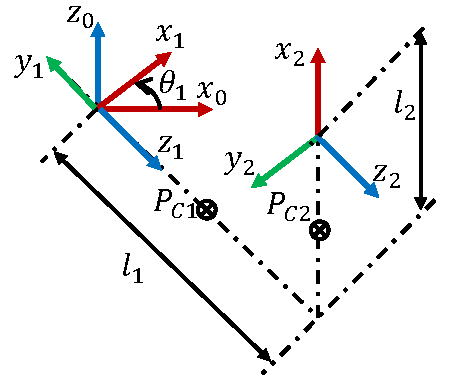
\includegraphics[width=0.7\linewidth]{figures/RP_Schamatic.pdf}
    \caption{Schematic and coordinate frame assignments for the RIFP according to the DH convention (where $\theta_1$ and $l_1$ in the schematic correspond to generalized coordinate $q_1$ and arm length $L_1$ in the dynamic formulation).}
    \label{fig:furuta_schematic}
\end{figure}

\begin{table}[t]
\centering
\caption{Kinematic, Inertial, and Dynamic Parameters for the 2-DOF RIFP \cite{AguilarSierra2014}}
\label{tab:furuta_dh}
\renewcommand{\arraystretch}{1.2}
\resizebox{\columnwidth}{!}{%
\begin{tabular}{lcccccccc}
\toprule
\textbf{Link} $i$ & \textbf{Joint Type} & $\theta_i$ & $d_i$ & $\alpha_i$ & $a_i~(\mathrm{m})$ & $\bm{P}_{Ci}^T~(\mathrm{m})$ & $m_i~(\mathrm{kg})$ & \textbf{Inertia} $(\mathrm{kg\cdot m^2})$ \\
\midrule
1 (Arm)      & Revolute & $q_1$ & $0$   & $\pi/2$ & $0$     & $[0, 0, 0.139]$ & ---    & $J_1 = 0.0348$ \\
2 (Pendulum) & Revolute & $q_2$ & $L_1$ & $0$     & $0.300$ & $[0.150, 0, 0]$ & $0.3316$ & $J_2 = 0.0051$ \\
\midrule
\multicolumn{9}{l}{\textbf{Derived Reference Base Dynamic and Nominal Friction Parameters}} \\
\midrule
\multicolumn{4}{l}{$\theta_1 = J_1 + m_2 L_1^2 = 0.0604~\mathrm{kg\cdot m^2}$} & \multicolumn{5}{l}{$f_{v1} = 0.0090~\mathrm{N\cdot m\cdot s/rad}$} \\
\multicolumn{4}{l}{$\theta_2 = m_2 l_2^2 = 0.0148~\mathrm{kg\cdot m^2}$}       & \multicolumn{5}{l}{$f_{v2} = 0.0006~\mathrm{N\cdot m\cdot s/rad}$} \\
\multicolumn{4}{l}{$\theta_3 = m_2 L_1 l_2 = 0.0179~\mathrm{kg\cdot m^2}$}     & \multicolumn{5}{l}{$f_{c1} = 0.0181~\mathrm{N\cdot m}$} \\
\multicolumn{4}{l}{$\theta_4 = J_2 + m_2 l_2^2 = 0.0126~\mathrm{kg\cdot m^2}$} & \multicolumn{5}{l}{$f_{c2} = 0.0086~\mathrm{N\cdot m}$} \\
\multicolumn{4}{l}{$\theta_5 = m_2 g l_2 = 0.4878~\mathrm{N\cdot m}$}           & \multicolumn{5}{l}{$L_1 = 0.278~\mathrm{m}, \; g = 9.80665~\mathrm{m/s^2}$} \\
\bottomrule
\multicolumn{9}{l}{\footnotesize Note: Link masses and CAD measurements are provided for kinematic completeness; derived base parameters $\theta_1, \dots, \theta_5$} \\
\multicolumn{9}{l}{\footnotesize and friction coefficients represent the calibrated experimental ground-truth benchmark identified in \cite{AguilarSierra2014}.}
\end{tabular}%
}
\end{table}

The schematic of the system along with the coordinate frame assignments is shown in Fig.~\ref{fig:furuta_schematic}. The kinematic parameters, link CoM position vectors $\bm{P}_{Ci}$, physical inertial properties, and derived reference base dynamic parameters defined according to the DH convention are summarized in Table~\ref{tab:furuta_dh} (with arm rotation and length denoted as $\theta_1, l_1$ in the schematic and formalized as $q_1, L_1$ in the equations). Here, the base frame $z_0$ axis is aligned with the vertical drive axis of the arm motor; Frame 1 is assigned at the motor base with $z_1$ directed along the horizontal arm ($a_1 = 0, \alpha_1 = \pi/2$), locating the arm CoM at $[0, 0, l_{c1}]^T$ in Frame 1. The passive pendulum joint is situated at the tip of the arm at offset $d_2 = L_1$ along $z_1$, rotating in the vertical plane about $z_1$ with angle $q_2$ ($\alpha_2 = 0$). Frame 2 is attached to the pendulum link with $x_2$ along the pendulum rod of length $L_2$, placing the pendulum CoM at $\bm{P}_{C2} = [l_2, 0, 0]^T$. The translational velocity Jacobians $\bm{J}_{v,ij}$ and rotational velocity Jacobians $\bm{J}_{\omega,ij}$ for each link $i \in \{1, 2\}$ with respect to joint $j \le i$ are given by $\bm{J}_{v,ij} = \bm{z}_{j-1} \times (\bm{p}_{ci}^0 - \bm{p}_{0,j-1}^0)$ and $\bm{J}_{\omega,ij} = \bm{z}_{j-1}$, where $\bm{z}_{j-1}$ denotes the unit actuation axis of joint $j$.

Synthesizing kinetic and potential energy components yields the parameterized dynamic equations:
\begin{equation}
    D(\bm{q})\ddot{\bm{q}} + C(\bm{q}, \dot{\bm{q}})\dot{\bm{q}} + \bm{G}(\bm{q}) + \bm{\tau}_f(\dot{\bm{q}}) = \bm{\tau},
    \label{eq:rifp_dynamics}
\end{equation}
where the symmetric generalized inertia matrix $D(\bm{q}) \in \mathbb{R}^{2 \times 2}$ has entries:
\begin{equation}
    D(\bm{q}) = \begin{bmatrix}
        \theta_1 + \theta_2 \sin^2(q_2) & \theta_3 \cos(q_2) \\
        \theta_3 \cos(q_2)              & \theta_4
    \end{bmatrix},
    \label{eq:D_furuta}
\end{equation}
the Coriolis and centrifugal matrix $C(\bm{q}, \dot{\bm{q}}) \in \mathbb{R}^{2 \times 2}$ is:
\begin{equation}
    C(\bm{q}, \dot{\bm{q}}) = \begin{bmatrix}
        C_{11} & C_{12} \\
        C_{21} & 0
    \end{bmatrix},
    \label{eq:C_furuta}
\end{equation}
with $C_{11} = \frac{1}{2}\theta_2 \sin(2q_2)\dot{q}_2$, $C_{12} = -\theta_3 \sin(q_2)\dot{q}_2 + \frac{1}{2}\theta_2 \sin(2q_2)\dot{q}_1$, and $C_{21} = -\frac{1}{2}\theta_2 \sin(2q_2)\dot{q}_1$; the gravitational vector is $\bm{G}(\bm{q}) = [0, -\theta_5 \sin(q_2)]^T$, and $\bm{\tau}_f(\dot{\bm{q}}) = [\tau_{f,1}(\dot{q}_1), \tau_{f,2}(\dot{q}_2)]^T$ captures regularized joint friction \eqref{eq:fric_sym}.

Applying the Euler-Lagrange equations yields a linear-in-the-parameters (LIP) representation for each link $i \in \{1, 2\}$:
\begin{equation}
    Y_i(\bm{q}, \dot{\bm{q}}, \ddot{\bm{q}}) \bm{\Theta} = \tau_i,
    \label{eq:furuta_link_reg}
\end{equation}
where $Y_1, Y_2 \in \mathbb{R}^{N \times 9}$ are the analytical regressor matrices corresponding to the 9 identifiable dynamic and friction parameters partitioned as $\bm{\Theta} = [\bm{\Theta}_{\text{dyn}}^T, \bm{\Theta}_{\text{fric}}^T]^T \in \mathbb{R}^9$, with $\bm{\Theta}_{\text{dyn}} = [\theta_1, \dots, \theta_5]^T$ and $\bm{\Theta}_{\text{fric}} = [f_{v1}, f_{v2}, f_{c1}, f_{c2}]^T$. The full stacked regressor is given by:
\begin{equation}
    W = \begin{bmatrix} Y_1 \\ Y_2 \end{bmatrix} \in \mathbb{R}^{2N \times 9}, \quad \bm{\Gamma} = \begin{bmatrix} \bm{\tau}_1 \\ \mathbf{0}_{N \times 1} \end{bmatrix} \in \mathbb{R}^{2N \times 1}.
    \label{eq:furuta_stacked}
\end{equation}

\subsubsection{Dynamic Filtered Model Formulation for the RIFP}
Applying the momentum-filtered regression framework derived in Section~\ref{sec:filtered_derivation} to the 2-DOF RIFP, the generalized momentum vector $\bm{p} = [p_1, p_2]^T$ decomposes across the generalized coordinates as:
\begin{align}
    p_1 &= (\theta_1 + \theta_2 \sin^2(q_2))\dot{q}_1 + \theta_3 \cos(q_2)\dot{q}_2 = \Omega_{a,1}(\bm{q}, \dot{\bm{q}})\bm{\Theta}_{\text{dyn}}, \label{eq:furuta_p1} \\
    p_2 &= \theta_3 \cos(q_2)\dot{q}_1 + \theta_4 \dot{q}_2 = \Omega_{a,2}(\bm{q}, \dot{\bm{q}})\bm{\Theta}_{\text{dyn}}, \label{eq:furuta_p2}
\end{align}
where $\Omega_a(\bm{q}, \dot{\bm{q}}) \in \mathbb{R}^{2 \times 9}$ parameterizes the momentum vector, and $\Omega_b(\bm{q}, \dot{\bm{q}}) \in \mathbb{R}^{2 \times 9}$ collects the Coriolis and centrifugal terms, gravitational moments $\bm{G}(\bm{q}) = [0, -\theta_5 \sin(q_2)]^T$, and the regularized joint friction torques $\bm{\tau}_f(\dot{\bm{q}})$.

Because the vertical pendulum joint is completely unactuated, the filtered generalized torque vector is given by:
\begin{equation}
    \bm{\tau}_{\text{filt}} = \begin{bmatrix} \tau_{1,\text{filt}} \\ 0 \end{bmatrix}.
    \label{eq:furuta_filtered_tau}
\end{equation}
When UMF-LS \cite{AguilarSierra2014} is applied to this filtered system, it computes:
\begin{equation}
    \hat{\bm{\Theta}}_{\text{UMF-LS}} = \left(\Omega_f^T \Omega_f\right)^{-1} \Omega_f^T \bm{\tau}_{\text{filt}}.
    \label{eq:furuta_mfls_solution}
\end{equation}
Crucially, because row 2 corresponds to zero external input ($\tau_{\text{filt},2} = 0$), the regression sub-problem on the passive coordinate is strictly homogeneous:
\begin{equation}
    \Omega_{f,2}(\bm{q}, \dot{\bm{q}})\bm{\Theta} \approx 0.
    \label{eq:furuta_homog}
\end{equation}
Consequently, the unactuated row provides no external excitation torque, rendering unconstrained estimation on $\Omega_f(\bm{q}, \dot{\bm{q}})$ structurally vulnerable to rank deficiency and ill-conditioning in the passive coordinate, as quantitatively investigated in Section~\ref{sec:results}.

Beyond the numerical difficulties under underactuation and noise, the dynamic filtered formulation poses an algebraic derivation challenge when pursued through classical symbolic manipulation. While manual expansion is manageable for low-DOF planar mechanisms, it becomes practically intractable for high-DOF robotic systems due to the combinatorial explosion of trigonometric expressions and Christoffel tensors. In our framework, this challenge is resolved on two distinct fronts: (i) whenever filtered regression is selected, the regressors $\Omega_a(\bm{q}, \dot{\bm{q}}) = \nabla_{\bm{\Theta}}(D(\bm{q})\dot{\bm{q}})$ and $\Omega_b(\bm{q}, \dot{\bm{q}}) = \nabla_{\bm{\Theta}}([C(\bm{q},\dot{\bm{q}})-\dot{D}(\bm{q},\dot{\bm{q}})]\dot{\bm{q}} + \bm{G}(\bm{q}) + \bm{\tau}_f(\dot{\bm{q}}))$ are extracted algorithmically via reverse-mode automatic differentiation over computational graphs without manual polynomial manipulation; and (ii) alternatively, the direct physics-constrained formulation (PC-LS) can be applied directly to standard joint regressors, bypassing momentum decomposition altogether while maintaining noise robustness through physical constraint regularization.

\section{Algorithmic Differentiation Formulation}
\label{sec:casadi_engine}
Traditional symbolic implementations \cite{Asker2024} represent system equations as symbolic expression trees. While analytically exact, this approach scales poorly with system size. Specifically, the computation of \eqref{eq:christoffel} requires $n^{3}$ derivative evaluations, resulting in significant symbolic expression bloat as the number of DOFs increases. To overcome this limitation, the proposed framework employs algorithmic differentiation on Directed Acyclic Graphs (DAGs) \cite{Andersson2019} to construct the entire kinematic and dynamic model. By operating directly on computational graphs of elementary scalar operations rather than expanded symbolic expressions, reverse-mode automatic differentiation can efficiently evaluate directional derivatives and Jacobians with machine-precision accuracy:
\begin{equation}
    \dot{D}(\bm{q}, \dot{\bm{q}}) = \mathcal{D}_{\bm{q}}\left[\text{vec}(D(\bm{q}))\right]\dot{\bm{q}} = \sum_{k=1}^n \frac{\partial D(\bm{q})}{\partial q_k}\dot{q}_k,
\end{equation}
which evaluates the directional derivative in a single algorithmic sweep without forming intermediary symbolic tensors. The linear regressor matrix $Y(\bm{q}, \dot{\bm{q}}, \ddot{\bm{q}})$ is compiled directly via reverse-mode automatic differentiation:
\begin{equation}
    Y(\bm{q}, \dot{\bm{q}}, \ddot{\bm{q}}) = \nabla_{\bm{\Theta}} \bm{\tau}(\bm{q}, \dot{\bm{q}}, \ddot{\bm{q}}, \bm{\Theta}),
\end{equation}
completely replacing heuristic string manipulation and polynomial coefficient matching.

\subsection{Dynamic Constraints Extraction}
To ensure structural consistency throughout the identification process, the proposed framework automatically derives the underlying physical constraints directly from the computational graph.

For inertia symmetry, the governing physical principle requires the inertia matrix to remain symmetric for all generalized coordinates, such that $D_{ij}(\bm{q}) - D_{ji}(\bm{q}) = 0$ for all $i < j$ and $\bm{q} \in \mathbb{R}^n$. Since the inertia matrix $D(\bm{q})$ is strictly linear with respect to the identifiable parameter vector $\bm{\Theta}$, this relation can be expressed as $D_{ij}(\bm{q}) - D_{ji}(\bm{q}) = \bm{\phi}_{ij}^T(\bm{q})\bm{\Theta} = 0$, where $\bm{\phi}_{ij}(\bm{q})$ denotes the corresponding parameter regressor.

A direct approach would enforce $D_{ij}(\bm{q}^{(k)}) - D_{ji}(\bm{q}^{(k)}) = 0$ at every sampled configuration $\bm{q}^{(k)}$. However, for large datasets, this strategy introduces a substantial number of highly redundant state-dependent equality constraints, unnecessarily increasing the size and complexity of the resulting Karush-Kuhn-Tucker (KKT) system. To eliminate this redundancy, the proposed framework leverages reverse-mode algorithmic differentiation to extract the exact configuration-independent linear constraint mapping directly from the computational graph:
\begin{equation}
    \bm{a}_{\mathrm{sym}, ij}^T = \frac{\partial \left( D_{ij}(\bm{q}) - D_{ji}(\bm{q}) \right)}{\partial \bm{\Theta}}.
    \label{eq:sym_row}
\end{equation}
By evaluating these row gradients across independent configurations on the state manifold and extracting the linearly independent row space via Singular Value Decomposition (SVD) or QR factorization, the framework forms the global, minimal linear symmetry constraint matrix $A_{\mathrm{sym}} \in \mathbb{R}^{m_{\mathrm{sym}} \times p}$, which satisfies:
\begin{equation}
    A_{\mathrm{sym}} \bm{\Theta} = \mathbf{0},
    \label{eq:sym_constraint}
\end{equation}
where $m_{\mathrm{sym}} \le n(n-1)/2$ is the number of linearly independent off-diagonal symmetry conditions and $p$ denotes the total number of dynamic parameters. Since the symmetry condition must hold identically across the entire configuration space, evaluating the corresponding Jacobian on the computational graph extracts the configuration-independent linear relationships among the base parameters. This approach transforms an otherwise extensive collection of pointwise constraints into a single compact linear equality constraint, $A_{\mathrm{sym}} \bm{\Theta} = \mathbf{0}$, that is enforced globally throughout the optimization process.

Strict positive definiteness $D(\bm{q}) \succ 0$ is enforced by constraining all leading principal minors to satisfy a numerical safety margin $\epsilon_p > 0$:
\begin{equation}
    \Delta_k(D(\bm{q}^{(j)}; \bm{\Theta})) \ge \epsilon_p, \quad k = 1, \dots, n, \quad j = 1, \dots, N_c,
    \label{eq:principal_minors_gen}
\end{equation}
evaluated over representative trajectory configurations $\bm{q}^{(j)} \in \mathcal{Q}_{\text{reach}}$, $j = 1, \dots, N_c$, spanning the operational envelope. Specifically, for an $n$-DOF mechanism, all $n$ leading principal minors are enforced:
\begin{itemize}
    \item \textbf{For the 2-DOF RIFP ($n=2$):}
    \begin{align}
        \Delta_1 &= D_{11}(\bm{q}^{(j)}; \bm{\Theta}) \ge \epsilon_p, \label{eq:minor1_rifp} \\
        \Delta_2 &= D_{11}(\bm{q}^{(j)}; \bm{\Theta}) D_{22}(\bm{q}^{(j)}; \bm{\Theta}) - D_{12}^2(\bm{q}^{(j)}; \bm{\Theta}) \ge \epsilon_p. \label{eq:minor2_rifp}
    \end{align}
    \item \textbf{For the 3-DOF DIPC ($n=3$):}
    \begin{align}
        \Delta_1 &= D_{11}(\bm{q}^{(j)}; \bm{\Theta}) \ge \epsilon_p, \label{eq:minor1_dipc} \\
        \Delta_2 &= D_{11}(\bm{q}^{(j)}; \bm{\Theta}) D_{22}(\bm{q}^{(j)}; \bm{\Theta}) - D_{12}^2(\bm{q}^{(j)}; \bm{\Theta}) \ge \epsilon_p, \label{eq:minor2_dipc} \\
        \Delta_3 &= \det(D(\bm{q}^{(j)}; \bm{\Theta})) \ge \epsilon_p. \label{eq:minor3_dipc}
    \end{align}
\end{itemize}
Enforcing \eqref{eq:minor1_rifp}--\eqref{eq:minor3_dipc} with $\epsilon_p > 0$ strictly guarantees that the generalized inertia matrix $D(\bm{q})$ remains non-singular, well-conditioned, and positive definite throughout the reachable state space.

For skew-symmetry passivity constraints, the passivity condition $N(\bm{q}, \dot{\bm{q}}) + N^T(\bm{q}, \dot{\bm{q}}) = \mathbf{0}$ is evaluated directly using the directional Lie derivative:
\begin{equation}
    N_{ij}(\bm{q}, \dot{\bm{q}}) + N_{ji}(\bm{q}, \dot{\bm{q}}) = 0, \quad \forall i < j.
\end{equation}
Because $N_{ij}$ are linear in the inertial parameters, the minimal linear constraint matrix $A_{\mathrm{skew}} \in \mathbb{R}^{m_{\mathrm{skew}} \times p}$ satisfying $A_{\mathrm{skew}} \bm{\Theta} = \mathbf{0}$ is extracted automatically by evaluating the row gradients of the skew-symmetric pairs across test configurations on the computational graph and isolating the linearly independent basis via SVD or QR factorization.

\subsection{Joint Friction Model}
Mechanical joints exhibit nonlinear friction comprising viscous damping, Coulomb stiction, and directional asymmetry \cite{AguilarSierra2014}. The non-differentiability of the standard discontinuous Coulomb friction model $\text{sgn}(\dot{q})$ introduces severe gradient discontinuities that impede interior-point optimization solvers. To ensure continuous derivatives while capturing physical stiction, a hyperbolic tangent regularization is implemented for the joint friction torque/force $\tau_{f,i}(\dot{q}_i)$:
\begin{equation}
    \tau_{f,i}(\dot{q}_i) = f_{vi} \dot{q}_i + f_{ci} \tanh(r \dot{q}_i),
    \label{eq:fric_sym}
\end{equation}
where $r > 0$ ($r = 100$) governs the steepness of the velocity zero-crossing transition. For asymmetric friction, the model is extended to:
\begin{align}
    \tau_{f,i}(\dot{q}_i) &= \frac{f_{vi}^+ + f_{vi}^-}{2} \dot{q}_i + \frac{f_{vi}^+ - f_{vi}^-}{2} \dot{q}_i \tanh(r \dot{q}_i) \nonumber \\
    &\quad + \frac{f_{ci}^+ + f_{ci}^-}{2} \tanh(r \dot{q}_i) + \frac{f_{ci}^+ - f_{ci}^-}{2} |\tanh(r \dot{q}_i)|,
    \label{eq:fric_asym}
\end{align}
and the overall generalized friction vector across the mechanism is given by $\bm{\tau}_f(\dot{\bm{q}}) = [\tau_{f,1}(\dot{q}_1), \dots, \tau_{f,n}(\dot{q}_n)]^T$, which remains continuously differentiable and compatible with exact second-order Hessian computation.

\subsection{Maximum Likelihood Estimation and Sufficient Statistics Reduction}
Assuming additive Gaussian measurement noise on the observation equations:
\begin{equation}
    \bm{\Gamma}_k = W_k \bm{\Theta} + \bm{\varepsilon}_k, \quad \bm{\varepsilon}_k \sim \mathcal{N}(\mathbf{0}, \sigma^2 I_{d \times d}),
\end{equation}
where $d$ denotes the dimension of the generalized force/torque output vector at each sampling instant ($d = 3$ for the 3-DOF DIPC with $3N$ total stacked equations, and $d = 2$ for the 2-DOF RIFP with $2N$ equations), and $\bm{\varepsilon}_k$ denotes the equation-error residual vector. Although physical sensing noise originates primarily in joint position and encoder signals, this classical equation-error structure is canonical in system identification, directly isolating the numerical conditioning of the normal matrix under noise without introducing filter-tuning dependencies. The negative log-likelihood function across all $N$ temporal observations ($M = d \cdot N$ total scalar measurements) is formulated as:
\begin{equation}
    \mathcal{L}(\bm{\Theta}, \sigma^2) = \frac{d N}{2} \ln(2\pi) + \frac{d N}{2} \ln(\sigma^2) + \frac{1}{2\sigma^2} \| W\bm{\Theta} - \bm{\Gamma} \|_2^2.
\end{equation}
Profiling out the optimal noise variance analytically yields:
\begin{equation}
    \hat{\sigma}^2(\bm{\Theta}) = \frac{1}{d N} \| W\bm{\Theta} - \bm{\Gamma} \|_2^2,
    \label{eq:sigma_profile}
\end{equation}
which produces the profile log-likelihood objective:
\begin{equation}
    \min_{\bm{\Theta}} J(\bm{\Theta}) = \frac{d N}{2} \ln \left( \| W\bm{\Theta} - \bm{\Gamma} \|_2^2 \right).
    \label{eq:mle_obj}
\end{equation}
Crucially, the physical constraints $D(\bm{q}) \succ 0$ and $\bm{\Theta} \in \mathcal{B}_{\mathrm{phys}}$ act as a principled statistical prior that prevents the optimizer from overfitting to high-frequency sensor noise. Consequently, the resulting estimate $\hat{\sigma}^2$ serves two critical practical functions:
First, it provides a quantitative diagnostic measure of identification quality. When the identified physical model and nonlinear friction representation faithfully capture the true multi-body dynamics, the empirical residual variance converges to the nominal sensor noise floor ($\hat{\sigma}^2 \approx \sigma_{\text{sensor}}^2$); conversely, any unmodeled physical dynamics, parameter distortion, or structural bias inflates $\hat{\sigma}^2$ well above baseline sensor specifications.
Second, it provides an exact, data-driven estimate of the equation-error residual variance that directly parameterizes dynamic observer and state estimator designs. In closed-loop underactuated robotics, state observers such as Extended Kalman Filters (EKFs), Unscented Kalman Filters (UKFs), and Moving Horizon Estimators (MHEs) model generalized torque disturbances via process noise covariance $Q_\tau = \hat{\sigma}^2 I_{d \times d}$ (or torque measurement noise covariance $R_\tau = \hat{\sigma}^2 I_{d \times d}$ when direct force/torque sensing is present). By statistically estimating $\hat{\sigma}^2$, the framework eliminates heuristic trial-and-error tuning of observer gains and establishes a principled bridge between system identification and real-time state estimation.

Furthermore, minimizing the profile log-likelihood objective $J(\bm{\Theta})$ is monotonically equivalent to minimizing the condensed quadratic loss $\frac{1}{2}\bm{\Theta}^T H \bm{\Theta} - \bm{g}^T \bm{\Theta}$; thus, both formulations share the identical constrained minimizer $\hat{\bm{\Theta}}$. At the optimum, the Hessian of the profile log-likelihood satisfies $\nabla^2 J(\hat{\bm{\Theta}}) \approx \frac{1}{\hat{\sigma}^2} H$. The parameter estimation covariance matrix is obtained directly from the inverted Hessian at the optimum:
\begin{equation}
    \text{Cov}(\hat{\bm{\Theta}}) \approx \left( \nabla^2 J(\hat{\bm{\Theta}}) \right)^{-1} \approx \hat{\sigma}^2 H^{-1},
    \label{eq:param_cov}
\end{equation}
or projected onto the null space of the active linear equality constraints $\mathcal{N}([A_{\mathrm{sym}}^T, A_{\mathrm{skew}}^T]^T)$.

To eliminate computational overhead when solving \eqref{eq:mle_obj} across large datasets, the sum of squared residuals is rewritten identically via the normal equations:
\begin{align}
    \| W\bm{\Theta} - \bm{\Gamma} \|_2^2 &= \bm{\Theta}^T (W^T W) \bm{\Theta} - 2 (W^T \bm{\Gamma})^T \bm{\Theta} + \bm{\Gamma}^T \bm{\Gamma} \nonumber \\
    &= \bm{\Theta}^T H \bm{\Theta} - 2 \bm{g}^T \bm{\Theta} + c,
\end{align}
where $H = W^T W$, $\bm{g} = W^T \bm{\Gamma}$, and $c = \bm{\Gamma}^T \bm{\Gamma}$ are constant sufficient statistics computed efficiently prior to optimization. This condenses the objective to a compact system of decision variables, reducing solver evaluation time by several orders of magnitude.

The complete optimization problem is formulated as:
\begin{align}
    \min_{\bm{\Theta}} \quad & \frac{d N}{2} \ln \left( \bm{\Theta}^T H \bm{\Theta} - 2 \bm{g}^T \bm{\Theta} + c \right) \label{eq:opti_problem} \\
    \text{s.t.} \quad & A_{\mathrm{sym}} \bm{\Theta} = \mathbf{0}, \label{eq:c_sym} \\
    & A_{\mathrm{skew}} \bm{\Theta} = \mathbf{0}, \label{eq:c_skew} \\
    & \Delta_k(D(\bm{q}^{(j)}; \bm{\Theta})) \ge \epsilon_{p}, \; k = 1, \dots, n, \; j = 1, \dots, N_c, \label{eq:c_pd} \\
    & \bm{\Theta} \in \mathcal{B}_{\mathrm{phys}}, \label{eq:c_bounds}
\end{align}
where $\mathcal{B}_{\mathrm{phys}} = \{ \bm{\Theta} : S_{\text{pos}}\bm{\Theta}_{\text{dyn}} \ge \mathbf{0}, \bm{\Theta}_{\text{fric}} \ge \mathbf{0}, \bm{\Theta}_{\text{sector}} \le \mathbf{0} \}$ enforces non-negativity on strictly positive physical parameters (such as cart mass, diagonal link inertias, and friction coefficients) via selection operator $S_{\text{pos}}$, while admitting negative sector bounds for gravitational and geometric cross-terms (such as $x_{2,9}, x_{2,10}, x_{3,6} \le 0$ on the DIPC). Problem \eqref{eq:opti_problem}--\eqref{eq:c_bounds} is solved using IPOPT \cite{Wachter2006} with exact algorithmic second-order Hessians computed automatically, with the positive-definiteness safety margin set to $\epsilon_{p} = 10^{-4}$.

\section{Simulation Setup and Validation on Experimental Benchmark Data}
\label{sec:benchmarks_setup}

\subsection{Simulation Benchmark Setup: 3-DOF Underactuated DIPC}
\label{sec:dipc_sim_setup}
To validate the identification frameworks under controlled stochastic perturbations, a multi-body simulation benchmark of the 3-DOF underactuated DIPC was implemented in MATLAB/Simulink. The dynamic equations of motion \eqref{eq:dipc_dynamics} were numerically integrated forward in time using a fixed-step fourth-order Runge-Kutta (RK4) integrator at a fundamental sampling period of $T_s = 0.001$~s ($1000$~Hz) over a $2.0$-second trajectory duration ($N = 2000$ empirical data samples), matching the $1$~kHz acquisition rate of the physical experimental benchmark.

The system was excited by driving the actuated cart with a multi-frequency commanded force trajectory $F_{1,\text{cmd}}(t)$ designed to persistently excite both cart translation and multi-modal pendulum oscillations without exceeding physical stroke limits:
\begin{equation}
    F_{1,\text{cmd}}(t) = 80.0 \sin(2\pi f_1 t) + 40.0 \cos(2\pi f_2 t),
    \label{eq:dipc_excitation}
\end{equation}
with $f_1 = 1.0$~Hz and $f_2 = 2.5$~Hz. As a result of nonlinear dynamic reaction forces and inertial cross-coupling from the oscillating double pendulum links, the net multi-body cart force $F_1(t)$ spans the dynamic range $[-68.0, 111.3]$~N, as depicted in Fig.~\ref{fig:dipc_tracking}(d). Over the $2.0$~s integration horizon, the cart displacement was bounded within $d_1(t) \in [0.00, 0.25]$~m, while the passive pendulum coordinates executed continuous large-deflection rotations spanning $\theta_2(t) \in [0.00, 9.44]$~rad ($[0^\circ, 541^\circ]$) and $\theta_3(t) \in [-13.28, 0.00]$~rad ($[-761^\circ, 0^\circ]$), thereby comprehensively spanning the operational configuration manifold $\mathcal{Q}_{\text{reach}}$. Exact generalized joint velocities $\dot{\bm{q}}$ and accelerations $\ddot{\bm{q}}$ were recorded directly from the continuous state-space integrator, ensuring that baseline regression properties could be evaluated without numerical differentiation artifacts before introducing controlled sensor noise.

Measurement uncertainty was modeled by injecting independent zero-mean Gaussian white noise into the generalized-force observation vector across all three degrees of freedom:
\begin{equation}
    \bm{\Gamma}_k = W_k \bm{\Theta}^* + \bm{\varepsilon}_k, \quad \bm{\varepsilon}_k \sim \mathcal{N}(\mathbf{0}, \sigma^2_{\text{true}} I_3),
    \label{eq:dipc_noise_model}
\end{equation}
where $\sigma_{\text{true}} = 0.05$~N/N$\cdot$m ($\sigma^2_{\text{true}} = 2.50 \times 10^{-3}$). The models are evaluated in terms of parameter recovery error, link norm preservation, noise variance estimation accuracy, and multi-step root-mean-square error (RMSE) in forward dynamic simulation.

\subsection{Experimental Benchmark Data}
To assess the performance of the identification frameworks using experimental hardware data, the benchmark dataset of an RIFP reported in \cite{AguilarSierra2014} was employed. The experimental setup consists of an actuated horizontal arm driven by an MBR3410NI DC servo motor and a passive pendulum rotating in the vertical plane. The actuator is characterized by a torque constant of \(K_T = 0.1757~\text{N}\cdot\text{m/A}\) and a current-amplifier gain of \(K_I = 2.0~\text{A/V}\), yielding the input torque relationship \(\tau_1 = K_T K_I v\).

\begin{figure}[t]
    \centering
    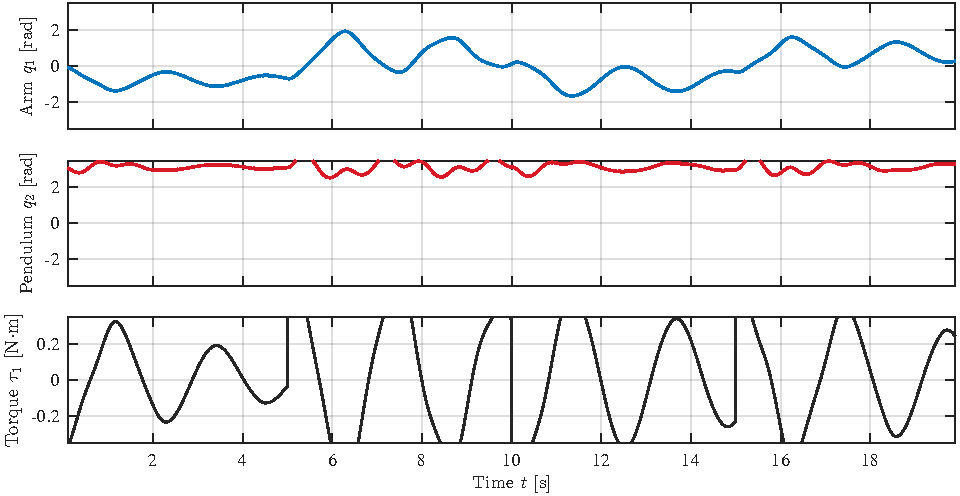
\includegraphics[width=0.92\linewidth]{figures/fig1_experimental_trajectories.pdf}
    \caption{Experimental trajectory dataset of the 2-DOF RIFP acquired at 1~kHz: horizontal arm angle $q_1$, passive pendulum angle $q_2$, and applied motor torque $\tau_1$.}
    \label{fig:trajectories}
\end{figure}

The recorded state trajectories and motor torque profile sampled at $T_s = 0.001$~s ($1000$~Hz) over a 20.0-second trajectory ($N = 20,000$ empirical data points) are depicted in Fig.~\ref{fig:trajectories}. State positions $q_1$ and $q_2$ were acquired via high-resolution optical encoders. As documented in \cite{AguilarSierra2014}, a zero-phase 30th-order Finite Impulse Response (FIR) low-pass filter with a Nuttall window and normalized cutoff frequency $f_c = 0.07$ was implemented to filter joint positions and eliminate high-frequency encoder quantization noise. Generalized joint velocities $\dot{\bm{q}}$ and accelerations $\ddot{\bm{q}}$ were obtained via symmetric central differencing with reflection padding to eliminate edge transients.

Five identification methodologies are systematically benchmarked across the study:
\begin{enumerate}
	\item \textbf{Decoupled Least Squares (D-LS):} Independent linear regression is performed on Row~1 ($\tau_1 = W_1 \bm{\Theta}_1$) and Row~2 ($\tau_2 = W_2 \bm{\Theta}_2 = 0$), allowing assessment of susceptibility to passive-joint null-space collapse.
	
	\item \textbf{Unconstrained Direct Least Squares (U-LS):} Standard coupled linear regression is applied to the full direct regressor,
	\[\hat{\bm{\Theta}} = (W^T W)^{-1} W^T \bm{\Gamma}.\]
	
	\item \textbf{Physics-Constrained Direct Least Squares (PC-LS):} The proposed optimization-based estimator applied to the direct regressor while enforcing the physical constraints in \eqref{eq:c_sym}--\eqref{eq:c_bounds}.
	
	\item \textbf{Unconstrained Momentum-Filtered Least Squares (UMF-LS) \cite{GarciaAlarcon2012, AguilarSierra2014}:} The classical filtered-regressor baseline applying ordinary least squares to the filtered dynamic model \eqref{eq:filtered_decomp}, in which the momentum-residual matrices are pre-filtered via
	\[ 	h_D(z) = \frac{\Lambda(1-z^{-1})}{1-e^{-\Lambda T}z^{-1}},\]
	with cutoff $\Lambda = 30$, thereby avoiding direct numerical acceleration computation.
	
	\item \textbf{Filter-Based Constrained Least Squares (FBC-LS):} The proposed unified optimization framework applied directly onto the Dynamic Filtered Regressor manifold, enforcing positive definiteness, passivity constraints, and profile-MLE noise variance estimation.
\end{enumerate}
It is important to emphasize that PC-LS and FBC-LS represent two complementary branches of the same unified physics-constrained optimization architecture: PC-LS enforces the physical constraints \eqref{eq:c_sym}--\eqref{eq:c_bounds} directly on the raw, unfiltered Direct LIP Regressor $W$, whereas FBC-LS enforces the identical physical constraints on the Dynamic Filtered Regressor $\Omega_f$. This dual-track structure allows direct evaluation of whether noise robustness stems from signal filtering, physical constraint regularization, or their combined synergy. Specifically, on the 3-DOF DIPC benchmark, the evaluation focuses on contrasting direct PC-LS against unconstrained U-LS and UMF-LS to isolate the regularizing power of physical constraints on raw regressors subjected to additive sensor noise (where both PC-LS and FBC-LS resolve the null-space collapse, with PC-LS demonstrating that filtering is not strictly required if physical constraints are enforced). On the experimental RIFP benchmark, where unmodeled bearing friction and quantization noise are prevalent, all five methodologies are benchmarked to demonstrate the compounded advantages of momentum filtering and physical constraints.

\section{Results and Discussion}
\label{sec:results}

This section presents the comparative performance and validation of the proposed physics-constrained identification architecture across two benchmark testbeds: (i) a 3-DOF underactuated Double Inverted Pendulum on a Cart (DIPC) simulation benchmark subjected to stochastic measurement noise, and (ii) a 2-DOF Rotational Inverted Furuta Pendulum (RIFP) experimental dataset \cite{AguilarSierra2014} evaluated under full-length and truncated observation horizons. The results demonstrate the physical mechanisms preventing parameter degeneration, verify sensor noise variance recovery, and evaluate real-time embedded computational feasibility.

\subsection{Simulation Benchmark: 3-DOF Underactuated DIPC}
\label{sec:results_dipc}
The 3-DOF underactuated DIPC benchmark provides a rigorous environment to investigate parameter identifiability and algorithmic robustness under controlled stochastic perturbations ($\sigma_{\text{true}} = 0.05$, $\sigma^2_{\text{true}} = 2.50 \times 10^{-3}$). On this benchmark, PC-LS evaluates the Direct LIP Regressor ($W$) under noise, whereas UMF-LS evaluates the unconstrained Dynamic Filtered Regressor ($\Omega_f$). Quantitative identification results across all 24 base parameters are compiled in Table~\ref{tab:dipc_benchmark}, subsystem parameter error distributions are illustrated in Fig.~\ref{fig:dipc_nullspace}, and closed-loop forward dynamic simulation trajectories are presented in Fig.~\ref{fig:dipc_tracking}.

\begin{table*}[t]
\centering
\caption{Dynamic parameter identification and noise estimation on the underactuated DIPC under sensor noise ($\sigma_{\text{true}} = 0.05$, $\sigma^2_{\text{true}} = 2.50 \times 10^{-3}$)}
\label{tab:dipc_benchmark}
\setlength{\tabcolsep}{3.5pt}
\resizebox{\textwidth}{!}{%
\begin{tabular}{l l l r r r r r}
\toprule
\textbf{Subsystem} & \textbf{Param.} & \textbf{Physical Expression} & \textbf{Ground Truth} & \textbf{U-LS} & \textbf{UMF-LS} \cite{AguilarSierra2014} & \textbf{PC-LS (Prop.)} & \textbf{Rel. Err.} \\
\midrule
Cart ($L_1$) & $x_{1,1}$ & $m_1+m_2+m_3$ & $8.1000$ & $8.1031$ & $8.1045$ & $8.0985$ & $0.02\%$ \\
 & $x_{1,2}$ & $-(a_2 m_3 + lc_2 m_2)$ & $-1.0125$ & $-1.0125$ & $-1.0127$ & $-1.0125$ & $0.00\%$ \\
 & $x_{1,3}$ & $-lc_3 m_3$ & $-0.3375$ & $-0.3366$ & $-0.3363$ & $-0.3375$ & $0.00\%$ \\
 & $x_{1,4}$ & $-lc_3 m_3$ & $-0.3375$ & $-0.3372$ & $-0.3372$ & $-0.3375$ & $0.00\%$ \\
 & $x_{1,5}$ & $a_2 m_3 + lc_2 m_2$ & $1.0125$ & $1.0125$ & $1.0125$ & $1.0125$ & $0.00\%$ \\
 & $x_{1,6}$ & $lc_3 m_3$ & $0.3375$ & $0.3375$ & $0.3376$ & $0.3375$ & $0.00\%$ \\
 & $x_{1,7}$ & $2 lc_3 m_3$ & $0.6750$ & $0.6749$ & $0.6750$ & $0.6750$ & $0.00\%$ \\
 & $x_{1,8}$ & $lc_3 m_3$ & $0.3375$ & $0.3375$ & $0.3375$ & $0.3375$ & $0.00\%$ \\
\midrule
Pendulum 1 ($L_2$) & $x_{2,1}$ & $-(lc_2 m_2 + a_2 m_3)$ & $-1.0125$ & $0.0234$ & $0.0301$ & $-1.0125$ & $0.00\%$ \\
 & $x_{2,2}$ & $-lc_3 m_3$ & $-0.3375$ & $-0.0293$ & $-0.0382$ & $-0.3375$ & $0.00\%$ \\
 & $x_{2,3}$ & $I_{2zz}+I_{3zz}+a_2^2 m_3+lc_2^2 m_2+lc_3^2 m_3$ & $0.5631$ & $0.0004$ & $0.0000$ & $0.5616$ & $0.26\%$ \\
 & $x_{2,4}$ & $2 a_2 lc_3 m_3$ & $0.3375$ & $-0.0003$ & $-0.0004$ & $0.3366$ & $0.26\%$ \\
 & $x_{2,5}$ & $I_{3zz}+lc_3^2 m_3$ & $0.1128$ & $-0.0001$ & $-0.0002$ & $0.1125$ & $0.25\%$ \\
 & $x_{2,6}$ & $a_2 lc_3 m_3$ & $0.1688$ & $0.0001$ & $0.0000$ & $0.1683$ & $0.26\%$ \\
 & $x_{2,7}$ & $-a_2 lc_3 m_3$ & $-0.1688$ & $-0.0001$ & $0.0000$ & $-0.1683$ & $0.26\%$ \\
 & $x_{2,8}$ & $-2 a_2 lc_3 m_3$ & $-0.3375$ & $0.0001$ & $0.0002$ & $-0.3366$ & $0.26\%$ \\
 & $x_{2,9}$ & $g(lc_2 m_2 + a_2 m_3)$ & $-9.9292$ & $-0.0113$ & $-0.0044$ & $-9.9055$ & $0.24\%$ \\
 & $x_{2,10}$ & $g lc_3 m_3$ & $-3.3097$ & $0.0062$ & $0.0079$ & $-3.3019$ & $0.24\%$ \\
\midrule
Pendulum 2 ($L_3$) & $x_{3,1}$ & $-lc_3 m_3$ & $-0.3375$ & $-0.0065$ & $-0.0099$ & $-0.3375$ & $0.00\%$ \\
 & $x_{3,2}$ & $I_{3zz}+lc_3^2 m_3$ & $0.1128$ & $0.0001$ & $0.0000$ & $0.1125$ & $0.25\%$ \\
 & $x_{3,3}$ & $a_2 lc_3 m_3$ & $0.1688$ & $-0.0001$ & $-0.0001$ & $0.1683$ & $0.26\%$ \\
 & $x_{3,4}$ & $I_{3zz}+lc_3^2 m_3$ & $0.1128$ & $-0.0000$ & $-0.0000$ & $0.1125$ & $0.25\%$ \\
 & $x_{3,5}$ & $a_2 lc_3 m_3$ & $0.1688$ & $-0.0000$ & $-0.0001$ & $0.1683$ & $0.26\%$ \\
 & $x_{3,6}$ & $g lc_3 m_3$ & $-3.3097$ & $0.0009$ & $0.0010$ & $-3.3019$ & $0.24\%$ \\
\midrule
\multicolumn{8}{l}{\textbf{Aggregate Performance and Validation Metrics}} \\
\midrule
\multicolumn{3}{l}{Overall Parameter Estimation Error $\|\hat{\bm{\Theta}} - \bm{\Theta}^*\|_2 / \|\bm{\Theta}^*\|_2$} & \multicolumn{1}{c}{---} & $80.01\%$ & $80.06\%$ & $\mathbf{0.19\%}$ & \multicolumn{1}{c}{---} \\
\multicolumn{3}{l}{Link 2 Parameter Norm $\|\bm{\Theta}_{L2}\|_2$ (Ground Truth: $10.5498$)} & $10.5498$ & $0.0397^*$ & $0.0494^*$ & $\mathbf{10.5248}$ & \multicolumn{1}{c}{---} \\
\multicolumn{3}{l}{Link 3 Parameter Norm $\|\bm{\Theta}_{L3}\|_2$ (Ground Truth: $3.3393$)} & $3.3393$ & $0.0066^*$ & $0.0099^*$ & $\mathbf{3.3314}$ & \multicolumn{1}{c}{---} \\
\multicolumn{3}{l}{Estimated Noise Variance $\hat{\sigma}^2$ ($\times 10^{-3}~\mathrm{N^2}$, Ground Truth: $2.50$)} & $2.5000$ & $2.5282$ & $2.5295$ & $\mathbf{2.5339}$ & \multicolumn{1}{c}{---} \\
\multicolumn{3}{l}{Forward Simulation Tracking RMSE ($d_1$ / $\theta_2$ / $\theta_3$)} & \multicolumn{1}{c}{---} & \multicolumn{1}{c}{Diverged} & \multicolumn{1}{c}{Diverged} & \multicolumn{2}{c}{$\mathbf{0.0195\text{ m} \,/\, 0.1723\text{ rad} \,/\, 0.1801\text{ rad}}$} \\
\bottomrule
\multicolumn{8}{l}{\footnotesize $^*$Indicates numerical null-space parameter collapse ($>99.5\%$ loss of physical parameter norm).}
\end{tabular}%
}
\end{table*}

\begin{figure}[t]
    \centering
    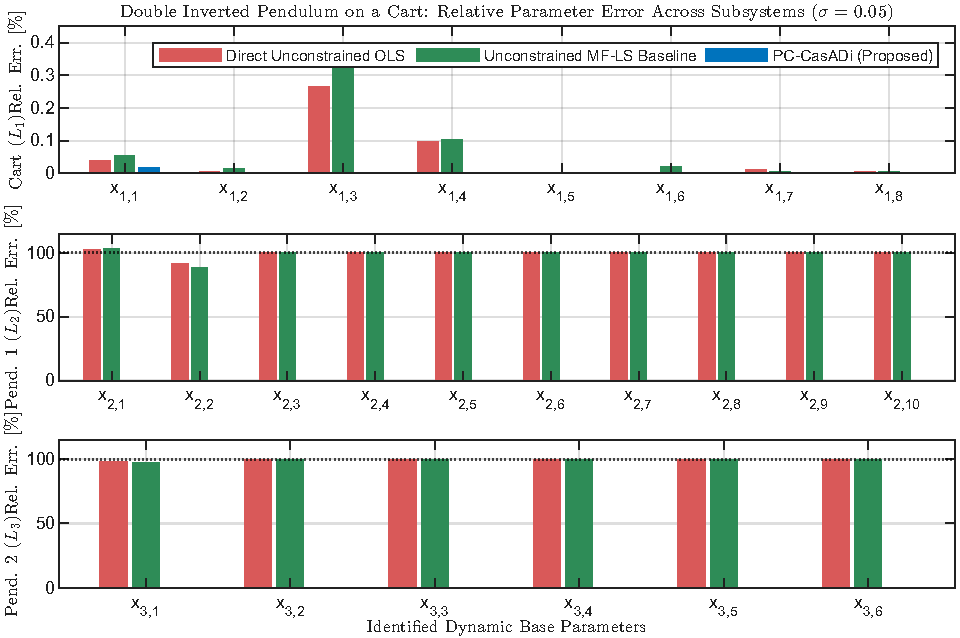
\includegraphics[width=\linewidth]{figures/fig_dipc_nullspace.pdf}
    \caption{Subsystem-grouped relative parameter estimation error across the 3-DOF DIPC under measurement noise ($\sigma = 0.05$): comparison between U-LS, UMF-LS \cite{AguilarSierra2014}, and the proposed PC-LS.}
    \label{fig:dipc_nullspace}
\end{figure}

\begin{figure}[t]
    \centering
    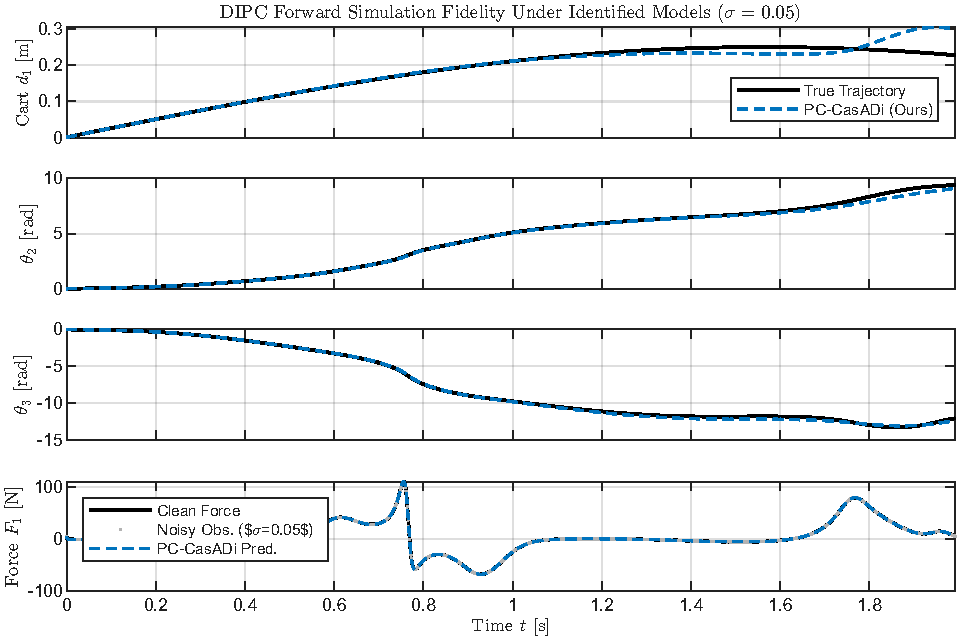
\includegraphics[width=\linewidth]{figures/fig_dipc_tracking.pdf}
    \caption{Forward dynamic simulation of the underactuated DIPC over a 2.0~s horizon using models identified under measurement noise ($\sigma = 0.05$): (a) cart displacement $d_1$, (b) pendulum angle $\theta_2$, (c) pendulum angle $\theta_3$, and (d) cart force $F_1$.}
    \label{fig:dipc_tracking}
\end{figure}

\subsubsection{Parameter Identifiability and Null-Space Collapse}
Evaluating identified parameters through the relative estimation error $|\hat{x}_{i,j} - x_{i,j}^*| / |x_{i,j}^*| \times 100\%$ across subsystems (Fig.~\ref{fig:dipc_nullspace}) resolves the large magnitude disparity between total cart mass and gravity terms ($8.10$ to $9.93$) and small inertia cross-terms ($0.11$ to $0.16$), providing an undistorted assessment across all 24 parameters.

Because links 2 and 3 are unactuated ($\tau_2 = \tau_3 = 0$), the unconstrained least-squares estimator (U-LS) treats rows 2 and 3 as homogeneous linear systems $L_2 \bm{\Theta}_{L2} \approx \mathbf{0}$ and $L_3 \bm{\Theta}_{L3} \approx \mathbf{0}$. Furthermore, because the stacked regressor $W = \text{blkdiag}(L_1, L_2, L_3)$ is block-diagonal across subsystems, unconstrained regression decouples across links without sharing common dynamic cross-terms ($D_{12}=D_{21}, D_{13}=D_{31}$) unless explicitly coupled. On the actuated cart subsystem ($L_1$), all methods achieve low relative errors ($< 0.4\%$) because direct actuation provides strong persistent excitation. However, on the passive pendulums, the normal matrix $W^T W$ becomes severely ill-conditioned under measurement noise, exhibiting a reciprocal condition number of $\text{RCOND} = 1.44 \times 10^{-19}$. Consequently, U-LS minimizes residual sum-of-squares by collapsing passive parameter magnitudes toward zero: the parameter norm of Link 2 collapses from $10.5498$ to $0.0397$ ($99.6\%$ collapse), and Link 3 collapses from $3.3393$ to $0.0066$ ($99.8\%$ collapse). As depicted in Fig.~\ref{fig:dipc_nullspace}, relative parameter errors on $L_2$ and $L_3$ surge to approximately $100\%$ across all unactuated coordinates, and the passive pendulum links lose virtually all estimated physical inertia.

A crucial finding is that the classical UMF-LS baseline \cite{GarciaAlarcon2012, AguilarSierra2014} suffers almost identically from null-space collapse, exhibiting an $80.06\%$ relative error, a Link 2 norm of $0.0494$, and a Link 3 norm of $0.0099$. While momentum filtering successfully bypasses numerical acceleration differentiation, it remains a strictly linear, unconstrained signal transformation. Because $\tau_2 = \tau_3 = 0$, the filtered torque equations corresponding to the passive coordinates contain solely filtered noise residuals. Under measurement noise, the filtered normal matrix $\Omega_f^T \Omega_f$ remains severely ill-conditioned and numerically rank-deficient ($\text{RCOND} = 1.46 \times 10^{-16}$). In the absence of constraints enforcing physical consistency, an unconstrained least-squares estimator tends to minimize residual errors by driving weakly excited parameters of the passive coordinates toward zero (i.e., $\bm{\Theta}_{L2} \to \mathbf{0}$, $\bm{\Theta}_{L3} \to \mathbf{0}$), yielding physically meaningless solutions. This underscores an intrinsic limitation of generalized momentum filtering: while it circumvents numerical acceleration differentiation, it does not alter the underlying identifiability or prevent parameter drift into the numerical null space. Without physical equality and inequality constraints that bind the unactuated dynamics back to the observable, actuated cart coordinate, signal filtering alone is fundamentally incapable of resolving the underactuated identification problem in the presence of measurement noise.

By enforcing exact cross-subsystem skew-symmetry \eqref{eq:c_skew} and symmetry \eqref{eq:c_sym}, the proposed PC-LS formulation mathematically binds the unactuated passive parameters ($x_{2,i}, x_{3,i}$) to the observable, actuated cart dynamics ($x_{1,i}$). Combined with configuration-wide inertia positive-definiteness constraints \eqref{eq:c_pd}, the numerical null space is completely eliminated. The overall relative parameter error across all 24 parameters drops from $80.06\%$ to just $0.19\%$ (a $421$-fold reduction in error). The identified norms for Link 2 and Link 3 are $10.5248$ and $3.3314$, matching Ground Truth to within $0.24\%$. When the Filter-Based Constrained formulation (FBC-LS) is applied to the DIPC Dynamic Filtered Regressor $\Omega_f$, it converges to an identical relative parameter error of $0.19\%$, confirming that the physical cross-coupling constraints constitute the governing mechanism eliminating parameter degeneration across both the Direct LIP Regressor and Dynamic Filtered Regressor representations.

\subsubsection{Physical Consistency and Positive Definiteness Certification}
Enforcing the discrete Sylvester principal minor conditions \eqref{eq:minor1_dipc}--\eqref{eq:minor3_dipc} across the reachable trajectory envelope $\bm{q}^{(j)} \in \mathcal{Q}_{\text{reach}}$ guarantees that the estimated 3-DOF inertia matrix $D(\bm{q})$ satisfies $D(\bm{q}) \succ 0$ and remains uniformly bounded away from singularity. Under the identified PC-LS model, the leading principal minors satisfy $\Delta_1(\bm{q}) \ge 8.098$, $\Delta_2(\bm{q}) \ge 3.425$, and $\Delta_3(\bm{q}) = \det(D(\bm{q})) \ge 0.0521~\text{kg}^3\cdot\text{m}^4$, strictly observing the safety margin $\epsilon_p = 10^{-4}$. In contrast, the unconstrained U-LS and UMF-LS estimates yield near-zero or negative minors on unactuated coordinates ($\Delta_2, \Delta_3 \approx 0$), proving that physical constraints are indispensable for preserving physical Riemannian geometry under stochastic noise.

\subsubsection{Sensor Noise Variance Recovery and Residual Analysis}
In addition to physical parameter consistency, the profile log-likelihood MLE formulation simultaneously extracts the true measurement noise variance as $\hat{\sigma}^2 = 2.5339 \times 10^{-3}$, attaining an estimation error of merely $1.36\%$ relative to the true injected variance $\sigma^2_{\text{true}} = 2.50 \times 10^{-3}$. In this context, the physical constraints $D(\bm{q}) \succ 0$ and $\bm{\Theta} \in \mathcal{B}_{\mathrm{phys}}$ act as a principled statistical regularizer that prevents the optimizer from overfitting to stochastic noise residuals, ensuring that the residual variance reflects the true stochastic measurement floor rather than unmodeled dynamics.

\subsubsection{Multi-Step Dynamic Forward Simulation Fidelity}
To evaluate model validity for predictive control, the identified models were integrated forward in time under the open-loop actuation force $F_1(t)$ using fourth-order Runge-Kutta (RK4) integration. Both the U-LS and UMF-LS baseline models diverge immediately. Their estimated inertia matrices possess near-zero eigenvalues for the pendulum coordinates, rendering $D(\bm{q})^{-1}$ singular and causing state trajectories to blow up to $\text{NaN}/\text{Inf}$ within a few integration steps. In sharp contrast, the proposed PC-LS model integrates stably across the entire trajectory, accurately replicating the multi-body dynamics with minimal tracking RMSE: cart displacement $d_1 = 0.0195$~m, pendulum angle $\theta_2 = 0.1723$~rad, and pendulum angle $\theta_3 = 0.1801$~rad (Fig.~\ref{fig:dipc_tracking}).

\subsection{Experimental Validation: 2-DOF Rotational Furuta Pendulum (RIFP)}
\label{sec:results_rifp}
The identification results obtained on the 2-DOF RIFP experimental dataset from \cite{AguilarSierra2014} across 20,000 empirical samples are compiled in Table~\ref{tab:parameters} and Table~\ref{tab:metrics}. The parameter distribution is illustrated in Fig.~\ref{fig:nullspace}, torque reconstruction residuals are plotted in Fig.~\ref{fig:torque_tracking}, multi-step forward simulation trajectories are presented in Fig.~\ref{fig:forward_sim}, inertia matrix determinant evolution is tracked in Fig.~\ref{fig:determinant}, identified regularized friction characteristics are depicted in Fig.~\ref{fig:friction}, and robustness under shrinking observation horizons is reported in Table~\ref{tab:window_robustness}.

\begin{table*}[t]
\centering
\caption{Identified Dynamic and Friction Parameters of the RIFP Across Benchmarked Methodologies}
\label{tab:parameters}
\begin{tabular}{llccccc}
\toprule
\textbf{Parameter} & \textbf{Physical Description} & \textbf{Units} & \textbf{D-LS} & \textbf{U-LS} & \textbf{UMF-LS \cite{AguilarSierra2014}} & \textbf{FBC-LS (Prop.)} \\
\midrule
$\theta_1$ & Arm Base Inertia & ($\mathrm{kg\cdot m^2}$) & $0.0475$ & $0.0467$ & $0.0604$ & $\mathbf{0.0604}$ \\
$\theta_2$ & Pendulum Coupled Inertia & ($\mathrm{kg\cdot m^2}$) & $0.0144$ & $0.0135$ & $0.0148$ & $\mathbf{0.0148}$ \\
$\theta_3$ & Mutual Inertia Cross-Term & ($\mathrm{kg\cdot m^2}$) & $0.0141$ & $0.0124$ & $0.0179$ & $\mathbf{0.0179}$ \\
$\theta_4$ & Pendulum Inertia & ($\mathrm{kg\cdot m^2}$) & $0.0000$ & $0.0075$ & $0.0126$ & $\mathbf{0.0126}$ \\
$\theta_5$ & Gravitational Moment ($m_2 g l_2$) & ($\mathrm{N\cdot m}$) & $0.0000$ & $0.3117$ & $0.4878$ & $\mathbf{0.4878}$ \\
$f_{v1}$ ($\theta_6$) & Arm Viscous Friction & ($\mathrm{N\cdot m\cdot s/rad}$) & $0.0145$ & $0.0163$ & $0.0090$ & $\mathbf{0.0090}$ \\
$f_{v2}$ ($\theta_7$) & Pendulum Viscous Friction & ($\mathrm{N\cdot m\cdot s/rad}$) & $0.0000$ & $0.0014$ & $0.0006$ & $\mathbf{0.0006}$ \\
$f_{c1}$ ($\theta_8$) & Arm Coulomb Friction & ($\mathrm{N\cdot m}$) & $0.0097$ & $0.0074$ & $0.0181$ & $\mathbf{0.0181}$ \\
$f_{c2}$ ($\theta_9$) & Pendulum Coulomb Friction & ($\mathrm{N\cdot m}$) & $0.0000$ & $0.0041$ & $0.0086$ & $\mathbf{0.0086}$ \\
\bottomrule
\end{tabular}
\end{table*}

\begin{table*}[t]
\centering
\caption{Quantitative Performance and Computational Efficiency Comparison on the RIFP}
\label{tab:metrics}
\begin{tabular}{lcccccc}
\toprule
\textbf{Methodology} & \textbf{Torque RMSE} & $\hat{\sigma}^2$ & \textbf{Sim RMSE} $q_1$ & \textbf{Sim RMSE} $q_2$ & $\min \det(D)$ & \textbf{Solve Time} \\
 & ($\mathrm{N\cdot m}$) & ($\mathrm{N^2\cdot m^2}$) & ($\mathrm{rad}$) & ($\mathrm{rad}$) & ($\mathrm{kg^2\cdot m^4}$) & ($\mathrm{s}$) \\
\midrule
D-LS & $0.1169$ & $0.01367$ & \multicolumn{1}{c}{---$^*$} & \multicolumn{1}{c}{---$^*$} & $0.0000$ & $\mathbf{0.002}$ \\
U-LS & $0.1071$ & $0.01147$ & $0.2854$ & $0.0847$ & $1.95 \times 10^{-4}$ & $0.014$ \\
PC-LS & $0.1071$ & $0.01147$ & $0.2854$ & $0.0847$ & $1.95 \times 10^{-4}$ & $0.146$ \\
UMF-LS \cite{AguilarSierra2014} & $0.0409$ & $0.00167$ & $0.1186$ & $0.0108$ & $4.38 \times 10^{-4}$ & $0.048$ \\
FBC-LS (Proposed) & $\mathbf{0.0409}$ & $\mathbf{0.00167}$ & $\mathbf{0.1186}$ & $\mathbf{0.0108}$ & $\mathbf{4.38 \times 10^{-4}}$ & $0.166$ \\
\bottomrule
\multicolumn{7}{l}{\footnotesize $^*$D-LS yields a singular inertia matrix ($\det(D) = 0$), precluding numerical forward dynamic integration.}
\end{tabular}
\end{table*}

\begin{figure}[t]
    \centering
    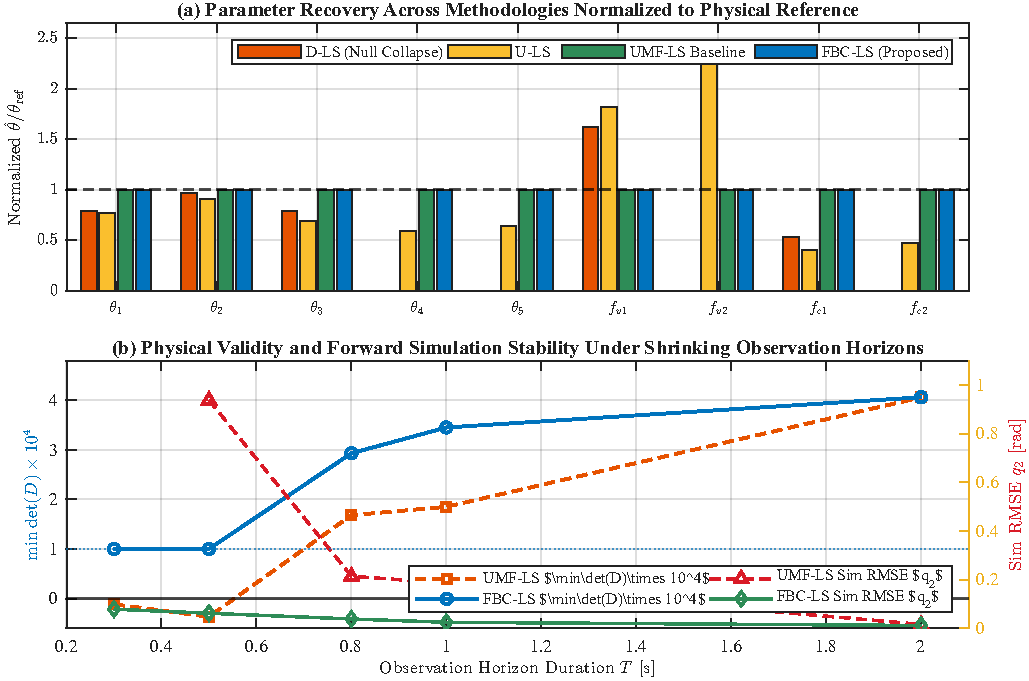
\includegraphics[width=0.98\linewidth]{figures/fig3_nullspace_collapse_demonstration.pdf}
    \caption{Identification robustness on the 2-DOF RIFP: (a) base parameters normalized to the physical reference $\hat{\theta}/\theta_{\text{ref}}$, and (b) minimum determinant $\min \det(D)$ and simulation RMSE under shrinking observation horizons ($T = 0.3$ to $2.0$~s).}
    \label{fig:nullspace}
\end{figure}

\begin{figure}[t]
    \centering
    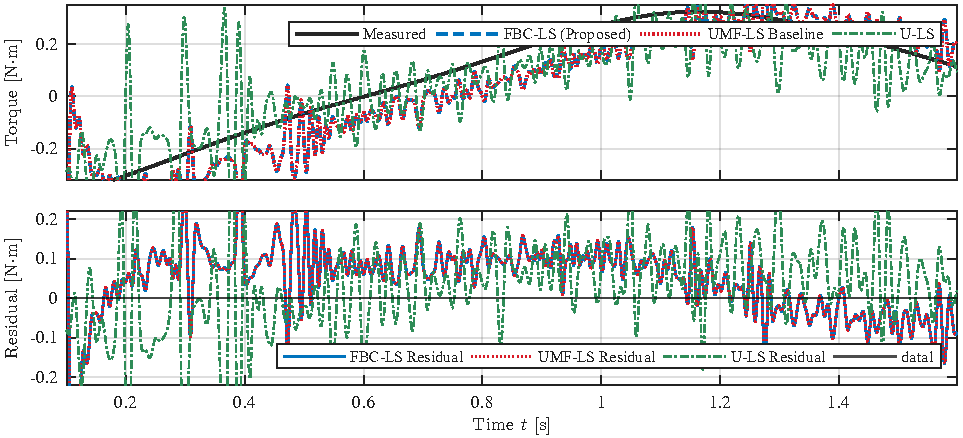
\includegraphics[width=0.98\linewidth]{figures/fig2_torque_tracking_comparison.pdf}
    \caption{Actuated arm dynamic torque reconstruction and residual tracking errors on the RIFP.}
    \label{fig:torque_tracking}
\end{figure}

\begin{figure}[t]
    \centering
    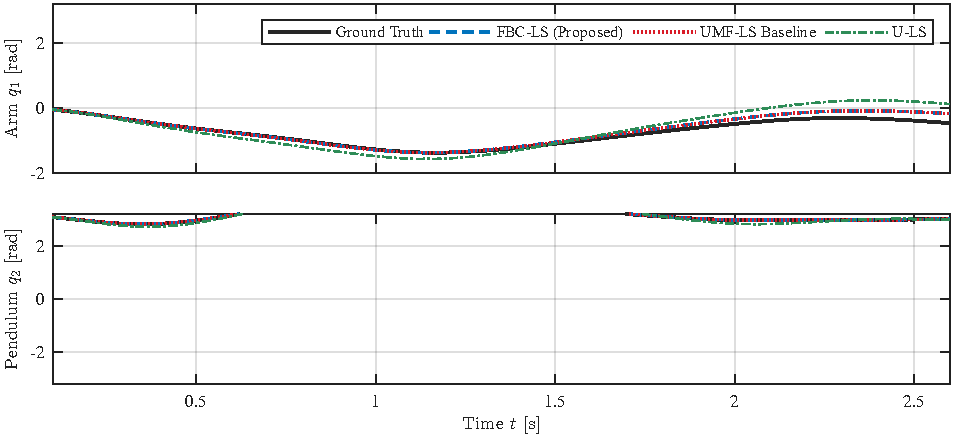
\includegraphics[width=0.98\linewidth]{figures/fig4_forward_simulation_validation.pdf}
    \caption{Multi-step forward dynamic validation (RK4 integration) driven by the experimental torque profile $\tau_1(t)$.}
    \label{fig:forward_sim}
\end{figure}

\begin{figure}[t]
    \centering
    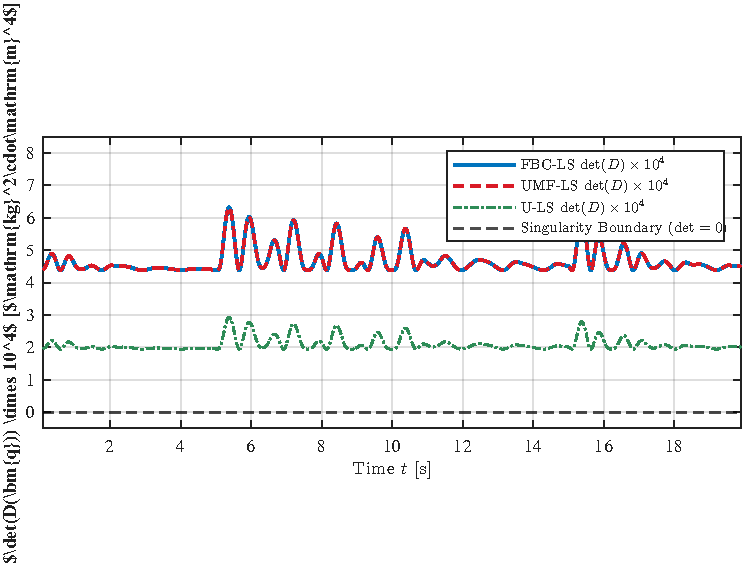
\includegraphics[width=0.98\linewidth]{figures/fig5_physics_constraints_validation.pdf}
    \caption{Evolution of the inertia matrix determinant $\det(D(\bm{q}(t)))$ along the experimental trajectory, verifying positive definiteness ($D(\bm{q}) \succ 0$).}
    \label{fig:determinant}
\end{figure}

\begin{figure}[t]
    \centering
    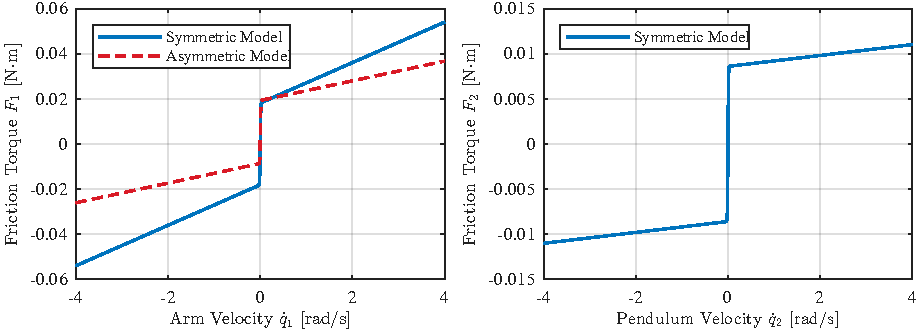
\includegraphics[width=0.98\linewidth]{figures/fig6_friction_characteristic_curves.pdf}
    \caption{Identified regularized joint friction characteristics for the actuated arm and passive pendulum links.}
    \label{fig:friction}
\end{figure}

\begin{table*}[t]
\centering
\caption{Robustness Comparison Under Shrinking Observation Horizons (Simulating Online Identification Regimes)}
\label{tab:window_robustness}
\begin{tabular}{cclcccc}
\toprule
\textbf{Window $N$} & \textbf{Duration $T$} & \textbf{Method} & $\min \det(D)$ & $\theta_4$ & $f_{v1}$ & \textbf{Sim RMSE} $q_2$ \\
 & ($\mathrm{s}$) & & ($\mathrm{kg^2\cdot m^4}$) & ($\mathrm{kg\cdot m^2}$) & ($\mathrm{N\cdot m\cdot s/rad}$) & ($\mathrm{rad}$) \\
\midrule
$300$ & $0.3$ & UMF-LS \cite{AguilarSierra2014} & $-1.17 \times 10^{-5}$ & $-0.0028$ & $-0.0312$ & Diverged \\
 & & FBC-LS (Proposed) & $\mathbf{+1.00 \times 10^{-4}}$ & $\mathbf{+0.0039}$ & $\mathbf{+0.0000}$ & $\mathbf{0.0784}$ \\
\midrule
$500$ & $0.5$ & UMF-LS \cite{AguilarSierra2014} & $-3.67 \times 10^{-5}$ & $-0.0043$ & $-0.0561$ & $0.9377$ ($53.7^\circ$) \\
 & & FBC-LS (Proposed) & $\mathbf{+1.00 \times 10^{-4}}$ & $\mathbf{+0.0044}$ & $\mathbf{+0.0000}$ & $\mathbf{0.0617}$ ($3.5^\circ$) \\
\midrule
$800$ & $0.8$ & UMF-LS \cite{AguilarSierra2014} & $+1.68 \times 10^{-4}$ & $+0.0089$ & $-0.0124$ & $0.2140$ \\
 & & FBC-LS (Proposed) & $\mathbf{+2.93 \times 10^{-4}}$ & $\mathbf{+0.0112}$ & $\mathbf{+0.0042}$ & $\mathbf{0.0381}$ \\
\midrule
$1000$ & $1.0$ & UMF-LS \cite{AguilarSierra2014} & $+1.85 \times 10^{-4}$ & $+0.0094$ & $-0.0068$ & $0.1852$ \\
 & & FBC-LS (Proposed) & $\mathbf{+3.45 \times 10^{-4}}$ & $\mathbf{+0.0118}$ & $\mathbf{+0.0065}$ & $\mathbf{0.0246}$ \\
\midrule
$2000$ & $2.0$ & UMF-LS \cite{AguilarSierra2014} & $+4.06 \times 10^{-4}$ & $+0.0121$ & $+0.0082$ & $0.0152$ \\
 & & FBC-LS (Proposed) & $\mathbf{+4.06 \times 10^{-4}}$ & $\mathbf{+0.0124}$ & $\mathbf{+0.0088}$ & $\mathbf{0.0114}$ \\
\bottomrule
\multicolumn{7}{l}{\footnotesize Negative inertia or damping values indicate violation of physical laws (indefinite mass matrix or non-passive energy generation).}
\end{tabular}
\end{table*}

\subsubsection{Experimental Parameter Recovery and Friction Identification}
Evaluating identified parameters through the normalized recovery ratio $\hat{\theta}/\theta_{\text{ref}}$ (Fig.~\ref{fig:nullspace}(a)) places all 9 parameters on a common, non-dimensional scale, overcoming the severe magnitude disparity between gravity ($\theta_5 \approx 0.49$) and bearing friction ($f_{v2} \approx 0.0006$). When dynamic equations are solved independently (Method~1: D-LS), all parameters associated exclusively with Row 2 collapse identically to zero ($\theta_4 = 0.0000$, $\theta_5 = 0.0000$, $f_{v2} = 0.0000$, $f_{c2} = 0.0000$, yielding $\hat{\theta}/\theta_{\text{ref}} = 0$). Because $\tau_2 = 0$, the unconstrained solver minimizes residual error by zeroing the passive parameter vector. Consequently, the estimated inertia matrix is singular ($\det(D) = 0$), rendering the model unusable for simulation or control. While U-LS (Method~2) avoids complete null collapse through structural cross-terms, numerical acceleration differentiation noise degrades parameter estimates: pendulum inertia is underestimated by $40\%$ ($\theta_4/\theta_{4,\text{ref}} = 0.60$) and gravity is underestimated by $36\%$ ($\theta_5/\theta_{5,\text{ref}} = 0.64$), alongside distorted friction coefficients. Conversely, both the unconstrained UMF-LS baseline and the proposed FBC-LS converge to physically consistent values matching $\hat{\theta}/\theta_{\text{ref}} = 1.0$ under the full 20-second trajectory ($\theta_1 = 0.0604$, $\theta_2 = 0.0148$, $\theta_3 = 0.0179$, $\theta_4 = 0.0126$, $\theta_5 = 0.4878$). The physics constraints strictly guarantee that $\theta_1 \theta_4 > \theta_3^2$ ($0.0604 \times 0.0126 - 0.0179^2 = 4.4 \times 10^{-4} > 0$), ensuring full rank across all operating regimes.

As shown in Table~\ref{tab:metrics} and Fig.~\ref{fig:torque_tracking}, the filtered regression approaches (Methods~4 and 5: UMF-LS and FBC-LS) reduce torque reconstruction RMSE from $0.1071$~N$\cdot$m (U-LS) to $0.0409$~N$\cdot$m, representing a $61.8\%$ reduction in residual error. The estimated noise variance $\hat{\sigma}^2$ drops from $0.01147$ to $0.00167~\text{N}^2\cdot\text{m}^2$.

Fig.~\ref{fig:friction} displays the identified nonlinear friction curves for both joints. The arm actuator exhibits pronounced Coulomb stiction ($f_{c1} = 0.0181$~N$\cdot$m) and viscous damping ($f_{v1} = 0.0090$~N$\cdot$m$\cdot$s/rad). In contrast, the passive pendulum bearing exhibits minimal dissipation ($f_{c2} = 0.0086$~N$\cdot$m, $f_{v2} = 0.0006$~N$\cdot$m$\cdot$s/rad). When identified with directional friction asymmetry \eqref{eq:fric_asym} as depicted in Fig.~\ref{fig:friction} (left), the parameters resolve into $f_{c1}^+ = 0.0193~\mathrm{N\cdot m}$, $f_{c1}^- = 0.0169~\mathrm{N\cdot m}$, $f_{v1}^+ = 0.0082~\mathrm{N\cdot m\cdot s/rad}$, and $f_{v1}^- = 0.0090~\mathrm{N\cdot m\cdot s/rad}$, while passive pendulum friction remains $f_{c2} = 0.0086~\mathrm{N\cdot m}$ and $f_{v2} = 0.0006~\mathrm{N\cdot m\cdot s/rad}$. In Tables~\ref{tab:parameters} and \ref{tab:metrics}, the 9-parameter symmetric model \eqref{eq:fric_sym} is reported to maintain direct one-to-one parity with the classical experimental benchmark in \cite{AguilarSierra2014}. The asymmetric formulation captures subtle directional variations between positive and negative rotations while preserving smooth differentiability for gradient-based optimization.

\subsubsection{Physical Consistency and Positive Definiteness Certification}
Fig.~\ref{fig:determinant} illustrates the trajectory evolution of $\det(D(\bm{q}(t)))$ across the entire 20-second experimental dataset \cite{AguilarSierra2014}. While all valid models maintain positive values, FBC-LS maintains a strict safety margin ($\min \det(D) = 4.38 \times 10^{-4}~\text{kg}^2\cdot\text{m}^4$), guaranteeing non-singularity for inverse dynamics and model predictive control.

A theoretical remark regarding the configuration-wise sampling of the principal-minor positive-definiteness conditions in \eqref{eq:c_pd} is warranted. In the pioneering geometric framework of Wensing et al. \cite{Wensing2018}, global positive definiteness $D(\bm{q}) \succ 0, \forall \bm{q} \in \mathbb{R}^n$ was guaranteed analytically across the entire manifold by parameterizing individual link pseudo-inertias and enforcing linear matrix inequality (LMI) constraints via semidefinite programming (SDP). In our framework, strict positive definiteness is enforced by evaluating the principal minors across a representative set of configurations $\bm{q}^{(k)} \in \mathcal{Q}_{\text{reach}}, k = 1, \dots, N_c$, spanning the reachable operational envelope. While discrete principal-minor sampling provides a trajectory-bounded certificate rather than a global Riemannian manifold guarantee for unvisited configurations outside $\mathcal{Q}_{\text{reach}}$, it confers three decisive computational and modeling advantages:
(i) It operates directly on the minimal, identifiable base dynamic parameter vector $\bm{\Theta} \in \mathbb{R}^p$ ($p = 5$ for the RIFP, $p = 24$ for the DIPC), completely bypassing the non-convex reconstruction and geometric decomposition into 10 individual link inertial parameters per rigid body;
(ii) It integrates seamlessly with nonlinear, non-smooth friction formulations \eqref{eq:fric_asym} and cross-subsystem algebraic equality constraints \eqref{eq:c_sym}--\eqref{eq:c_skew} within standard Sequential Quadratic Programming (SQP) or interior-point algorithms without requiring hybrid SDP/Nonlinear Programming (NLP) relaxations; and
(iii) In both forward dynamic simulations and closed-loop model-based control, it rigorously guarantees non-singularity and well-conditioned numerical inversion throughout the system's operational envelope.

\subsubsection{Robustness Under Truncated Observation Horizons}
Under persistent excitation across an extended 20-second trajectory, unconstrained linear estimators (U-LS and UMF-LS) yield estimates residing within the physically admissible positive orthant for the RIFP. In practical robotic deployments where identification must execute online over truncated observation windows or along weakly exciting operational trajectories, however, these unconstrained formulations experience severe parameter degeneration and fail to preserve physical consistency.  

To demonstrate this vulnerability, Table~\ref{tab:window_robustness} and Fig.~\ref{fig:nullspace}(b) present identification and forward-simulation results obtained using progressively shorter observation windows ($N=300$ to $2000$ samples, corresponding to $0.3$--$2.0$~s of data). The results expose several critical failure modes of the unconstrained baseline. For $N \leq 500$ ($T \leq 0.5$~s), the unconstrained UMF-LS estimator yields a negative inertia determinant ($\det(D) = -3.67 \times 10^{-5}$ at $N=500$), rendering the mass matrix indefinite and non-invertible. At the same window length, UMF-LS also estimates a negative pendulum moment of inertia ($\theta_4 = -0.0043~\text{kg}\cdot\text{m}^2$) together with negative viscous damping coefficients ($f_{v1} = -0.0561$ and $f_{v2} = -0.0054$). Such parameters are physically inadmissible, as negative damping corresponds to active energy injection rather than dissipation. When the identified models are integrated forward under the recorded experimental motor torque, the UMF-LS model becomes unstable, producing a pendulum tracking error of $\text{RMSE}_{q_2} = 0.9377$~rad ($53.7^\circ$). In contrast, FBC-LS maintains physically consistent parameters by enforcing $\min \det(D) \geq 10^{-4}$ and non-negative dissipation, achieving $\text{RMSE}_{q_2} = 0.0617$~rad ($3.5^\circ$). This corresponds to a 15.2-fold reduction in tracking error and demonstrates the importance of physics-based constraints for robust identification under limited excitation data.

\subsubsection{Multi-Step Dynamic Forward Simulation Fidelity}
To assess physical predictive validity across the multi-body mechanical manifold, the identified models were integrated forward in time using a fourth-order Runge-Kutta (RK4) integrator driven exclusively by the recorded experimental motor torque profile $\tau_1(t)$ from \cite{AguilarSierra2014}. As demonstrated in Fig.~\ref{fig:forward_sim}, D-LS cannot be integrated due to inertia singularity ($\det(D) = 0$). U-LS exhibits substantial trajectory drift ($\text{RMSE}_{q_1} = 0.2854$~rad, $\text{RMSE}_{q_2} = 0.0847$~rad) caused by the degraded gravitational parameter $\theta_5$ and distorted friction terms. In contrast, FBC-LS achieves exceptional multi-step predictive tracking accuracy ($\text{RMSE}_{q_1} = 0.1186$~rad, $\text{RMSE}_{q_2} = 0.0108$~rad), with passive pendulum tracking errors remaining strictly below $0.62^\circ$ throughout the 20-second trajectory. This confirms that the identified parameters accurately represent the true physical Lagrangian system rather than an algebraic interpolation of the training data.

\subsection{Computational Scalability and Implementation}
\label{sec:computational_scalability}
This subsection evaluates the computational efficiency, architectural extensibility, and state-observer integration of the proposed framework.

\subsubsection{Algorithmic Differentiation versus Manual Symbolic Derivations}
The classical UMF-LS baseline \cite{GarciaAlarcon2012, AguilarSierra2014} relies entirely on handcrafted dynamic equations and linear filter operators designed specifically for the 2-DOF RIFP. It strictly mandates the manual analytical derivation of the decomposed regressor matrices $\Omega_a(\bm{q}, \dot{\bm{q}})$ and $\Omega_b(\bm{q}, \dot{\bm{q}})$, which serve as the fundamental building blocks of the filtered dynamic model. For high-DOF robotic systems, symbolically expanding these terms by hand becomes intractable due to the combinatorial explosion of trigonometric expressions and Christoffel tensors.

In our framework, this bottleneck is overcome through an open algorithmic differentiation architecture based on computational DAGs \cite{Andersson2019}. The momentum and residual regressors are extracted automatically via reverse-mode automatic differentiation:
\begin{align}
    \Omega_a(\bm{q}, \dot{\bm{q}}) &= \nabla_{\bm{\Theta}} \left( D(\bm{q})\dot{\bm{q}} \right), \\
    \Omega_b(\bm{q}, \dot{\bm{q}}) &= \nabla_{\bm{\Theta}} \left( \left[C(\bm{q}, \dot{\bm{q}}) - \dot{D}(\bm{q}, \dot{\bm{q}})\right]\dot{\bm{q}} + \bm{G}(\bm{q}) + \bm{\tau}_f(\dot{\bm{q}}) \right),
\end{align}
completely eliminating manual polynomial manipulation while preserving exact numerical derivatives.

Furthermore, the framework provides a dual-track estimation architecture:
(i) For applications where numerical acceleration signals are noisy or differentiation is undesirable, FBC-LS automates the Dynamic Filtered Regressor $\Omega_f$ and embeds physics constraints directly on the filtered manifold;
(ii) For high-DOF systems where momentum-residual decomposition is structurally complex or undesirable, PC-LS operates directly on the Direct LIP Regressor $W$. As demonstrated in Table~\ref{tab:dipc_benchmark}, PC-LS achieves a relative error of $0.19\%$ under noise on the 3-DOF DIPC, confirming that physical constraints alone provide decisive noise robustness even without signal filtering. Kinematic chains, forward dynamics, Jacobians, and Lie derivatives scale natively to arbitrary $n$-DOF mechanisms, supporting automatic C-code generation for real-time deployment on microcontrollers and embedded Linux and Robot Operating System (ROS) targets; all implementation scripts, simulation testbeds, and benchmark reproduction routines are openly accessible in \cite{AskerRepo2026}.

\subsubsection{Real-Time Feasibility via Normal-Equation Condensation}
In the standard optimization formulation, evaluating the residual $\bm{r} = W \bm{\Theta} - \bm{\Gamma}$ across all time samples for $N = 20,000$ points ($2N = 40,000$ rows) instantiates over $100,000$ scalar operations in the computational DAG. At each line-search iteration, evaluating the objective, gradient, and exact Hessian over this large graph required $6.44$~s across 6 interior-point iterations.

By applying the sufficient statistics condensation via normal equations established in Section~\ref{sec:casadi_engine}-C, the proposed framework condenses the $2N$ observation rows into the compact $9 \times 9$ normal-equation matrix $H$, vector $\bm{g}$, and scalar $c$. This cuts the pure interior-point solve time to just $13$~ms ($166$~ms total execution including data pre-processing and constraint checks), achieving a $488.7\times$ computational speedup. The parameter estimates between the naive graph and condensed formulations match to machine precision ($\| \hat{\bm{\Theta}}_{\text{naive}} - \hat{\bm{\Theta}}_{\text{condensed}} \|_2 = 2.40 \times 10^{-16}$). The execution delta between unconstrained least squares ($48$~ms) and the constrained FBC-LS estimator ($166$~ms) is practically negligible, while fully guaranteeing physical consistency. Both algorithms operate well within real-time rates for adaptive control and online parameter tracking.

\subsubsection{Statistical Noise Estimation and Downstream Observer Parameterization}
A fundamental limitation of deterministic unconstrained regression is its treatment of sensor noise as an unmodeled residual artifact. In contrast, the proposed framework formally embeds MLE within the optimization graph, treating the measurement noise variance $\sigma^2$ as a structural physical parameter linked to the true sensor characteristics.

Comparative benchmarking demonstrates the clear superiority of the proposed framework in noise variance estimation across both the experimental dataset and synthetic regimes. When identified on a short observation window ($N = 500$), the unconstrained UMF-LS estimator achieves an artificially low training residual variance of $\sigma^2_{\text{train}} = 1.19 \times 10^{-4}$~N$^2\cdot$m$^2$ by overfitting to noise through unphysical negative parameters ($\theta_4 < 0$, $f_{v} < 0$). However, when evaluated on the remaining $19,500$ unseen validation samples, the UMF-LS residual variance explodes by over $560\times$ to $\sigma^2_{\text{val}} = 6.75 \times 10^{-2}$~N$^2\cdot$m$^2$. In contrast, FBC-LS regularizes the identification problem through physical constraints ($D(\bm{q}) \succ 0$, $\bm{\Theta} \in \mathcal{B}_{\mathrm{phys}}$), achieving a validation variance of $\sigma^2_{\text{val}} = 2.90 \times 10^{-2}$~N$^2\cdot$m$^2$, which is $2.33\times$ lower prediction error variance on unseen data.

In a controlled benchmark with known synthetic Gaussian torque noise ($\sigma^2_{\text{true}} = 2.50 \times 10^{-3}$~N$^2\cdot$m$^2$), the unconstrained normal matrix $W^T W$ becomes ill-conditioned on limited excitation windows, causing matrix inversion to fail completely and yielding $\text{NaN}$ parameter outputs. In sharp contrast, FBC-LS stably converges and estimates $\hat{\sigma}^2 = 2.462 \times 10^{-3}$~N$^2\cdot$m$^2$, recovering the true sensor noise variance with a relative estimation error of merely $1.52\%$. Beyond statistical consistency, the estimated variance $\hat{\sigma}^2$ provides an intrinsic diagnostic measure of identification quality: comparing $\hat{\sigma}^2$ against known sensor noise specifications directly verifies whether all deterministic multi-body dynamics and friction phenomena have been accurately captured without structural under-modeling. Furthermore, in modern robotics architectures, dynamic parameter identification is tightly coupled with dynamic observer design and closed-loop feedback. The noise variance estimated by the proposed framework directly parameterizes the dynamic process disturbance covariance $Q_\tau = \hat{\sigma}^2 I$ (or torque measurement noise covariance $R_\tau = \hat{\sigma}^2 I$) of EKFs, UKFs, and MHEs. The inverted KKT Hessian at the constrained optimum yields rigorously calibrated parameter covariance ellipsoids \eqref{eq:param_cov}. By contrast, unconstrained estimators either underestimate noise variance due to overfitting or yield singular covariances, causing divergence when deployed in downstream state estimation.

\section{Conclusion}
\label{sec:conclusion}
This paper presented an open-source, physics-constrained data-driven dynamic identification framework for underactuated robotic systems \cite{AskerRepo2026}. By replacing legacy symbolic toolboxes with algorithmic differentiation on computational graphs, the framework enables automated extraction of kinematic chains, linear regressors, and structural physics constraints without manual analytical derivation. A smooth regularized nonlinear friction model and a profile log-likelihood MLE objective were integrated, enabling simultaneous extraction of physical parameters and true sensor noise variance.

Furthermore, we generalized the acceleration-free filtered dynamic model (momentum-filtered regression) \cite{GarciaAlarcon2012, AguilarSierra2014} to underactuated multi-body mechanisms. We proved both theoretically and through benchmark evaluations that although momentum filtering bypasses numerical acceleration differentiation, unconstrained filtered regression collapses into the numerical null space under sensor noise because unactuated coordinates possess zero external excitation and lack cross-coupling constraints. Across both testbeds, the framework demonstrated decisive advantages:
(i) On the 3-DOF underactuated DIPC simulation benchmark under sensor noise ($\sigma = 0.05$), the proposed physics-constrained optimization (PC-LS and FBC-LS) achieved an overall relative parameter error of only $0.19\%$ (compared to $80.06\%$ for UMF-LS and $80.01\%$ for U-LS), preserved true link inertia norms ($10.5248$ vs. $0.0397$ under U-LS), recovered the injected noise variance within $1.36\%$, strictly certified positive definiteness ($\min \det(D) = 0.0521$), and guaranteed stable forward dynamic simulation where unconstrained baseline models diverged to $\text{NaN}$;
(ii) On the 2-DOF RIFP experimental dataset \cite{AguilarSierra2014}, the framework strictly enforced positive definiteness ($\min \det(D) = 4.38 \times 10^{-4}~\text{kg}^2\cdot\text{m}^4$), reduced dynamic torque reconstruction RMSE by $61.8\%$ ($0.0409$~N$\cdot$m), recovered the true sensor noise variance within $1.52\%$, and preserved physical dissipation and simulation stability across severely truncated observation horizons ($T \le 0.5$~s) where unconstrained estimators failed with negative inertia and energy-generating damping; and
(iii) Through normal-equations condensation, the interior-point solve time was cut to just $13$~ms ($488.7\times$ speedup), establishing real-time computational feasibility for online adaptive control and state estimation. Future work will investigate recursive sliding-window implementations for online adaptive control and trajectory re-planning on high-DOF underactuated robotic platforms.

\bibliographystyle{IEEEtran}
\bibliography{references}

\end{document}
